%% Document class
\documentclass[final,3p,times,twocolumn]{elsarticle}    % two column format
% \documentclass[preprint,review,12pt]{elsarticle}        % one column format

%% Use package
\usepackage{graphicx}
\usepackage{epstopdf}
\usepackage{amssymb}
\usepackage{amsthm}
\usepackage{amsmath}
\usepackage{latexsym}
\usepackage{mathrsfs}
\usepackage[tight,nice]{units}
\usepackage{harpoon}
\usepackage{chemarrow}
\usepackage{lineno}
\usepackage{harpoon}
\usepackage{chemarrow}
\usepackage{lscape}
\usepackage{color}
\usepackage{lineno}
\usepackage{colortbl}
\usepackage{chngcntr}
\usepackage{etoolbox}
\usepackage{tikz}
\usepackage{enumitem}
\usepackage{float}
\usepackage{soul}
\usepackage{url}
\usepackage{xr}

% Figure sizes
% Full textwidth for this template is ~ 6.47in
% A single column width for the template is ~ 3.07in

%% Submittal Material - Moves all figures to end of document
% \usepackage{endfloat}

%% Bib options
\biboptions{sort&compress}

%% Cross referencing option
\makeatletter
\newcommand*{\addFileDependency}[1]{
    \typeout{(#1)}
    \@addtofilelist{#1}
    \IfFileExists{#1}{}{\typeout{No file #1.}}  }

\makeatother
\newcommand*{\myexternaldocument}[1]{
    \externaldocument{#1} 
    \addFileDependency{#1.tex} 
    \addFileDependency{#1.aux}  }
    
\myexternaldocument{supplementary}

%% Eliminates automatic footer note
\makeatletter
\def\ps@pprintTitle{%
  \let\@oddhead\@empty
  \let\@evenhead\@empty
  \let\@oddfoot\@empty
  \let\@evenfoot\@oddfoot
}

%% Specific Journal 
% \journal{Journal Name}

%% Begin document
\begin{document}

%%%%%%%%%%%%%%%%%%%%%%%%%%%%%%%%%%%%%%%%%%%%%%%%%%%%%%%%%%%%%%%%%%%%%%%%%%
%% Begin Frontmatter
\begin{frontmatter}

\title{Predicted Impacts of Pt and Ionomer Distributions \\ 
       on Low Pt-loaded PEMFC Performance}

\author[CSM]{Corey R. Randall}
\author[CSM]{Steven C. DeCaluwe \corref{cor}}
\cortext[cor]{Corresponding Author: Tel: (303) 273-3666}
\ead{decaluwe@mines.edu}
        
\address[CSM]{Colorado School of Mines, 1500 Illinois St, Golden, CO 80401}

%%%%%%%%%%%%%%%%%%%%%%%%%%%%%%%%%%%%%%%%%%%%%%%%%%%%%%%%%%%%%%%%%%%%%%%%%%
\begin{abstract} 
Low-cost proton exchange membrane fuel cells (PEMFCs) with high performance and durability have been difficult to develop due to limited understanding of complex physiochemical processes in the cathode catalyst layer (CL). PEMFCs fabricated with low Pt loadings suffer cell losses beyond those predicted due solely to reduced catalyst surface area. Although there is a consensus that these additional losses involve thin ionomer films in the cathode CL, a precise, mechanistic explanation for the limiting processes remains elusive. In this publication, we present a physically based model with novel structure-property relationships for the nano-thin Nafion films in the cathode CL. The model also includes two-phase transport to predict the influence of pore flooding. Results suggest that flooding exacerbates the low Pt surface areas in low loading PEMFCs such that a shift in Faradaic current distribution occurs at much lower current densities than cells with high loadings. As current density increases, protons must travel further into the CL. This results in higher Ohmic overpotentials caused by ion transport resistance in the Nafion ionomer. We also present a parametric study of the CL microstructure to identify designs which prevent flooding and reduce Ohmic overpotentials. We find that graded Pt and ionomer loadings reduce Ohmic overpotentials and flooding, but individually do not provide significant improvements. However, a dual graded CL (i.e., both Pt and ionomer are graded) is predicted to significantly improve the maximum power density and limiting current compared to uniformly loaded CLs. The results from this work highlight the importance of accurate transport parameters for thin-film Nafion and provide a pathway to future low-cost PEMFCs via precise control of cathode CL microstructures.
\end{abstract}

\begin{keyword}
Proton exchange membrane fuel cells \sep structure-property relationships \sep low Pt loading \sep numerical modeling \sep catalyst layer microstructure \sep Cantera
\end{keyword}

\end{frontmatter}

%%%%%%%%%%%%%%%%%%%%%%%%%%%%%%%%%%%%%%%%%%%%%%%%%%%%%%%%%%%%%%%%%%%%%%%%%%
\section{Introduction}

Proton exchange membrane fuel cells (PEMFCs) are a promising clean energy technology. However, wide-spread PEMFC adoption requires lower-cost cells that meet performance and durability requirements. Currently, low-cost PEMFC performance is limited by the use of an expensive Pt catalyst, which accounts for roughly half of the stack cost~\cite{bib:kongkanand_2016, bib:xie_2021}. Cost reductions via lower Pt loadings lead to poor PEMFC performance~\cite{bib:sakai_2009, bib:ohma_2011, bib:leimin_2009, bib:harzer_2018, bib:banham_2021}. For example, Owejan et al.~\cite{bib:owejan_2013} found that reducing the Pt loading from 0.2 to 0.025~mg$_{\rm Pt}$~cm$^{-2}$ lowered the maximum power density of an air-fed PEMFC from 1.26 to 0.86~W~cm$^{-2}$ -- a 32\% decrease. These losses exceed those expected due solely to reduced Pt surface area. Research suggests that these unexplained performance losses are linked to transport through catalyst layer (CL) ionomer~\cite{bib:paul_2011, bib:paul_2014, bib:weber_2014, bib:modestino_2013, bib:jung_2013}.

Nano-thin Nafion films in PEMFC CLs provide ionic pathways for protons moving between the membrane and the Pt catalyst surface. Molecular oxygen and water also absorb into Nafion as they move between CL pores and Pt catalysts. Quantifying the potential losses associated with each process is challenging for current experimental capabilities, leading to limited understanding of complex physiochemical interactions in the CL~\cite{bib:weber_2014, bib:modestino_2013, bib:jung_2013}. Some research suggests surface resistance to oxygen transport at Nafion-gas or Nafion-Pt interfaces as a limiting phenomena~\cite{bib:weber_kusoglu_2014, bib:nonoyama_2011, bib:kongkanand_2016}, but contradictory experimental results have also been published~\cite{bib:liu_2015}. In general, concrete evidence for a mechanistic explanation for limiting CL phenomena with low Pt loading remains elusive.

Numerical models can further our understanding of limiting cathode processes, by resolving and predicting species concentrations, fluxes, and reaction rates, providing insights beyond what current experiments allow. For example, previous modeling studies helped identify limitations due to pore flooding, motivating the use of hydrophobic, high-porosity cathode GDLs~\cite{bib:chu_2003, bib:abdollahzadeh_2014, bib:weber_darling_2004}. In addition, models help identify design improvements. Exercising models by varying operating conditions and design parameters can identify design rules and principles more rapidly than prototyping and experiments~\cite{bib:weber_2014, bib:arif_2020}. 

Leveraging the benefits of physically informed models, however, requires predictive capabilities, which in turn rely on accurate property and process parameters (e.g., transport parameters, reaction rate coefficients, etc.). Previous thin-film Nafion experiments provide in-situ measurements of total water uptake~\cite{bib:kongkanand_2011, bib:bharath_2016, bib:dura_2009, bib:decaluwe_2018} and nano-structures~\cite{bib:dura_2009, bib:decaluwe_2018, bib:wood_2009, bib:peltonen_2021}. However, dynamic \emph{operando} measurements that provide proton conductivity and/or oxygen diffusion are sparse or entirely lacking from literature. While the studies that do provide these transport parameters are helpful~\cite{bib:chen_2019, bib:paul_mccreery_2014}, the thicknesses and substrates used are not always relevant to operating PEMFC CLs. 

In this work, we use a pseudo-2D Newman-type model to identify PEMFC limitations in devices with low Pt loading. The model includes two-phase molecular transport, chemical and charge-transfer reactions, and ion transport. The model implements realistic transport properties for oxygen diffusion and proton transport through nano-thin Nafion films. Transport properties are derived from two sources: quantitative structural data from neutron reflectometry experiments~\cite{bib:decaluwe_2018} and ionic conductivity measurements~\cite{bib:paul_mccreery_2014}. These relationships enable transport parameters that vary with local ionomer loading, Pt loading, Nafion-phase water volume fraction, and temperature. 

Results presented include model validation against experimental results with Pt loadings between 0.025 and 0.2~mg~cm$^{-2}$, followed by a parametric study of the CL microstructure. Varied parameters include: CL thickness, ionomer loading, and Pt distribution. We also model novel graded microstructures, where the Pt and/or ionomer loading vary with CL depth (lower near the gas diffusion layer (GDL) and higher near the proton exchange membrane (PEM)), to limit pore flooding and Ohmic losses. Results demonstrate that grading the ionomer reduces flooding and directly improves limiting current. A dual graded CL (where Pt and ionomer both vary) predicted the highest performance of all modeled designs, with a 25\% increase in maximum power density and a 15\% increase in limiting current compared to uniformly loaded CLs.


%%%%%%%%%%%%%%%%%%%%%%%%%%%%%%%%%%%%%%%%%%%%%%%%%%%%%%%%%%%%%%%%%%%%%%%%%%
\section{Model framework}
\label{sect:model-framework}

\begin{figure*}
    \centering
    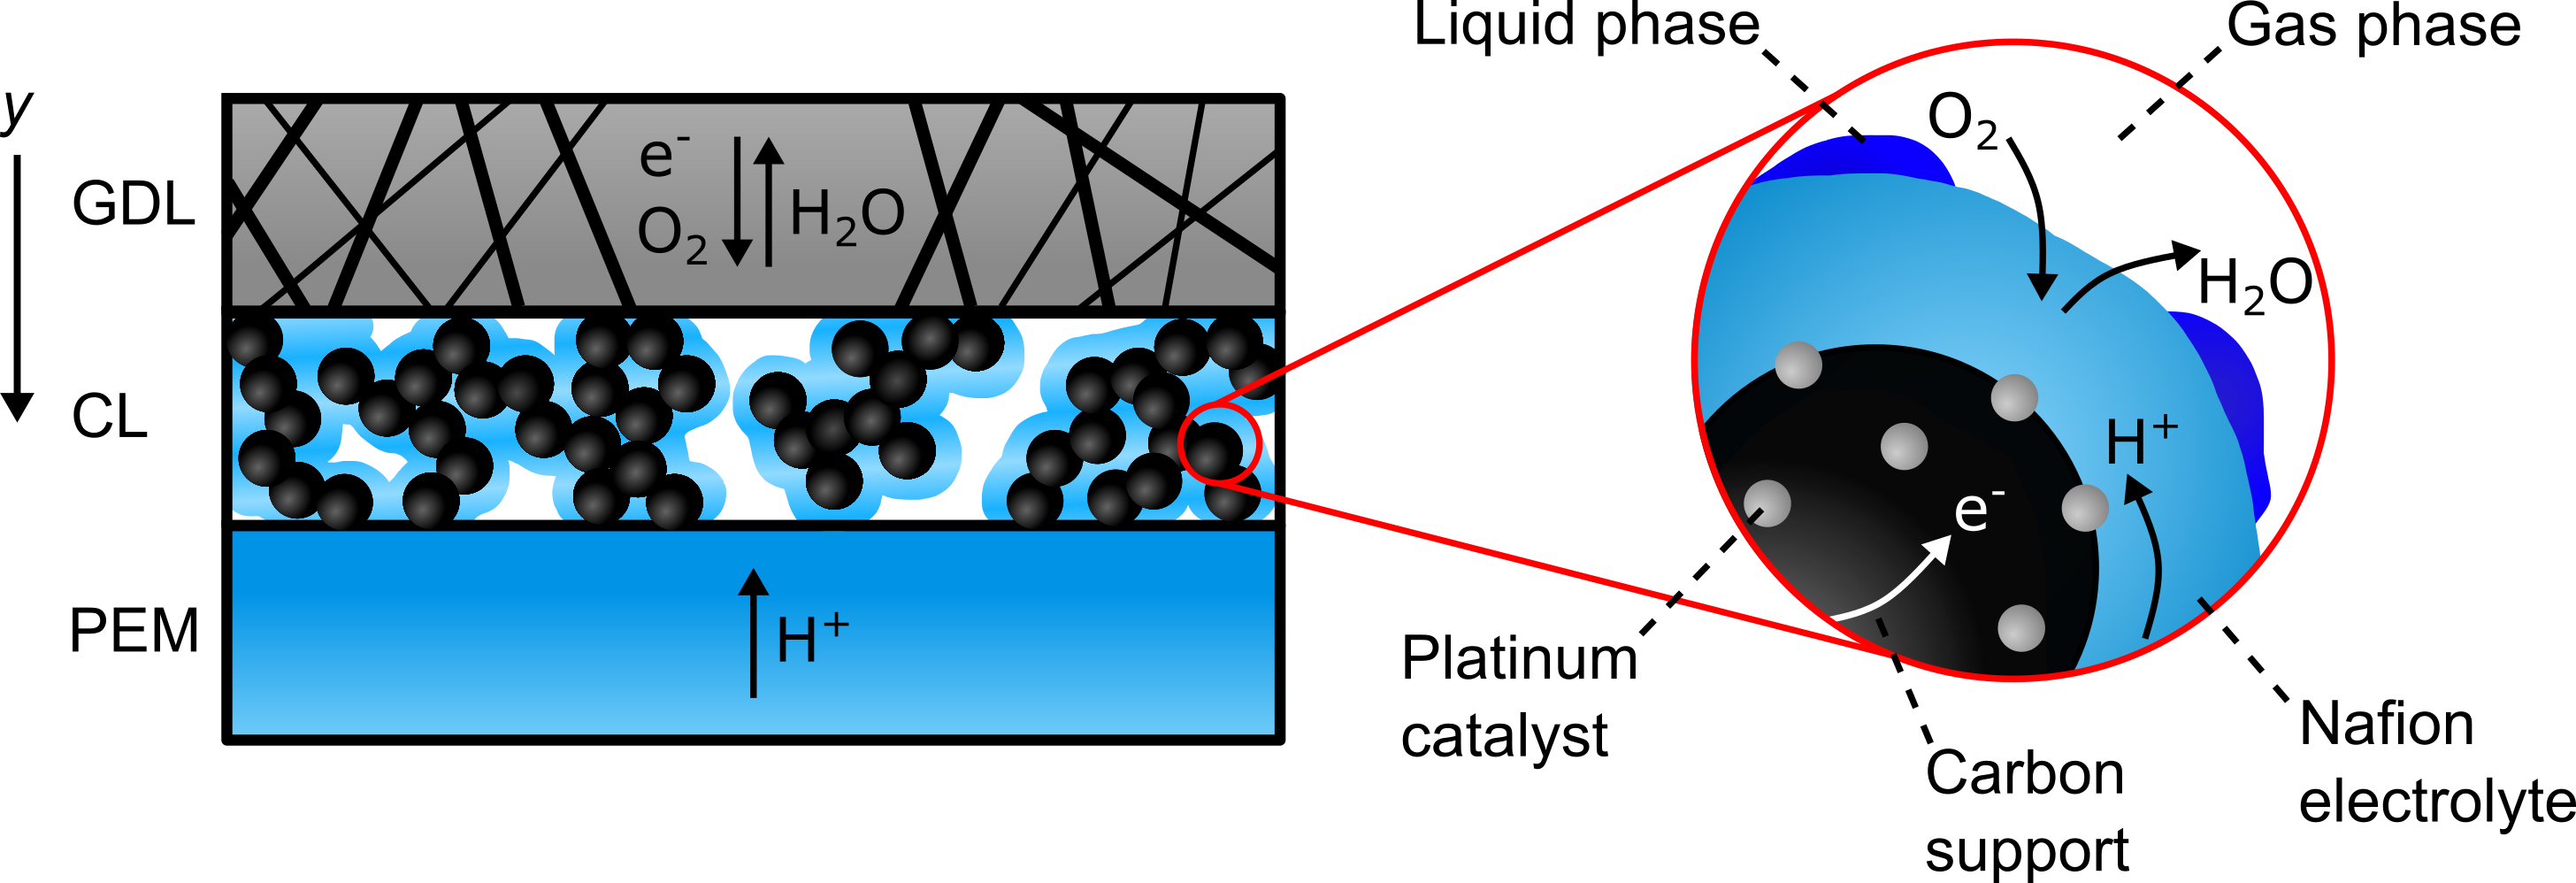
\includegraphics[width=5.825in]{figures/core-shell-5_825in.png}
    \caption{Representation of the modeled domain and physical processes. The model includes discretized domains for the gas diffusion layer (GDL) and catalyst layer (CL). The proton exchange membrane (PEM) is treated as a linear resistor and is not discretized. The positive $y$-direction (i.e. depth) is oriented toward the PEM.}
    \label{fig:core-shell}
\end{figure*}

The model presented here is a pseudo-2D PEMFC model focused primarily on resolving limiting cathode processes. The model domain, illustrated in figure~\ref{fig:core-shell}, includes the cathode GDL and CL, with a simple linear resistor PEM and an ideal reversible anode. The cathode GDL and CL are discretized, and governing equations that conserve mass, elements, and charge are solved using finite-volume methods. The following sections provide the time derivatives used for the state variables. These variables are initialized and integrated as a function of time until steady-state is reached. Repeated integrations over a range of user-defined current densities generates polarization curves for comparison against experimental data. 

\subsection{Model assumptions}
The model assumes that:

\begin{enumerate}[label=(\roman*.)]
    \item The entire domain is isothermal,
    \item Ionomer electric potentials vary only as a function of CL depth ($y$),
    \item Carbon and Pt phases in the cathode have uniform electric potential throughout the CL,
    \item Nafion-liquid and Nafion-gas interfacial areas are linearly dependent on local water saturation (${\cal S}_{\rm w}$),
    \item Representative domains within each volume are spherical solids with Pt-decorated carbon cores, coated by Nafion shells of uniform thickness.
\end{enumerate}

The geometry represented in figure~\ref{fig:core-shell} uses a minimal number of experimentally informed inputs including carbon radius ($r_{\rm c}$), Nafion shell thickness ($t_{\rm N}$), Pt radius ($r_{\rm Pt}$), and dry porosity ($\epsilon_{\rm g}^{\rm o}$). For the current study, these inputs are determined from representative transmission electron microscope images~\cite{bib:he_2005}. Other geometric parameters required for the model are derived from this base set. These include interfacial reaction areas, Nafion-phase volume fraction, tortuosity factors, etc. Derivation details are available in the supplementary information (SI).

\subsection{Gas-phase mass conservation}

The mass densities of each gas-phase species $k$ ($\rho_{k,\rm g}$) are used to track the state of the gas. Given a constant temperature from assumption (i.), this fixes the gas state (the total density $\rho_{\rm g} = \sum \rho_{k,\rm g}$ and the mass fractions $Y_{k,\rm g} = \rho_{k,\rm g} / \rho_{\rm g}$). The evolution of $\rho_{k,\rm g}$ with time is dependent upon the mass flux (${\bf J}_{k,\rm g}$, kg~m$^{-2}_{\rm tot}$~s$^{-1}$) with neighboring volumes and local net molar production rates ($\dot{s}_{k,m}$, kmol~m$^{-2}$~s$^{-1}$) for interfacial reactions at the gas-phase interface with condensed phase $m$ (solid or liquid). The governing equation for gas-phase species is:
\begin{equation} \label{eq:mass-cons-gas}
    \frac{d \rho_{k,\rm g}}{d t} = \frac{1}{\epsilon_{\rm g}} \left[ 
    - \nabla \cdot \mathbf{J}_{k,\rm g} + \rho_{k,\rm g} \frac{d \epsilon_{\rm w}}{d t}
    + \sum_m \dot{s}_{k,m} W_k A_m \right],
\end{equation}
where $\epsilon_{\rm g}$ and $\epsilon_{\rm w}$ are the gas-phase and liquid-phase volume fractions. The term involving the liquid-phase volume fraction captures compressive effects from pore flooding (solved via equation~\ref{eq:volfrac_w}). The molecular weights are $W_k$ (kg~kmol$^{-1}$) and specific surface area for phase $m$ is $A_m$ (m$^2$~m$^{-3}_{\rm tot}$). The sum is over all $m$ phases which have a gas-phase interface.

The gas-phase mass flux includes advective and diffusive terms: 
\begin{equation} \label{eq:mass-flux}
    \mathbf{J}_{k,\rm g} = -\frac{\rho_{k,\rm g} K_{\rm g}}{\mu_{\rm g}} \nabla P_{\rm g} 
                  -\frac{\epsilon_{\rm g}}{\tau_{\rm fac,\,g}} D_{k,\rm g} 
                   \rho_{\rm g} \nabla Y_{k,\rm g}.
\end{equation}
The advective term is driven by local gradients in gas-phase pressure $P_{\rm g}$. Here, $K_{\rm g}$ and $\mu_{\rm g}$ are the effective permeability and viscosity of the gas phase, respectively. Fick's law is used for the diffusive term, accounting for gradients in mass fractions $Y_{k,\rm g}$, where $\epsilon_{\rm g}$ is the gas-phase volume fraction and $\tau_{\rm fac,\,g}$ the toruosity factor, calculated via a Bruggeman correlation with an exponent of $-0.5$~\cite{bib:bruggeman_1935}. The standard diffusion coefficients ($D_{k,\rm g}$) are calculated using a mixed-species transport model, as described in~\cite{bib:kee_2018}. Chemical kinetic routines for calculating $\dot{s}_{k,m}$ are discussed in section~\ref{sect:kinetics}.

\subsection{Liquid-phase mass conservation}

The liquid phase is treated as pure liquid water. This phase influences other model processes (e.g. Nafion-gas and Nafion-liquid interfacial reactions) due to localized flooding. The volume fraction of the liquid phase ($\epsilon_{\rm w}$) changes in time according to:
\begin{equation}\label{eq:volfrac_w}
    \frac{d \epsilon_{\rm w}}{d t} = \hat{V}_{\rm w} \left[ 
    - \nabla \cdot {\bf N}_{\rm w} + \sum_m \dot{s}_{{\rm w},m} A_m \right].
\end{equation}
Here, $\hat{V}_{\rm w}$ and ${\bf N}_{\rm w}$ are the molar volume (m$^3$~kmol$^{-1}$) and molar flux (kmol~m$^{-2}_{\rm tot}$~s$^{-1}$) of liquid water. The molar flux comes from Darcy's law:
\begin{equation} \label{eq:darcy-liquid}
    {\bf N}_{\rm w} = -\frac{C_{\rm w} K_{\rm w}}{\mu_{\rm w}} \nabla P_{\rm w}.
\end{equation}
In equation~(\ref{eq:darcy-liquid}), the molar density of the liquid water phase $C_{\rm w}$ (kmol~m$^{-3}_{\rm tot}$), effective permeability of the liquid phase $K_{\rm w}$ (m$^{2}_{\rm tot}$), and liquid water viscosity $\mu_{\rm w}$ (Pa~s), are multiplied by the gradient in liquid-phase pressure $P_{\rm w}$ (Pa), which is defined using the gas-phase pressure and capillary pressure $P_{\rm c}$ (Pa),
\begin{equation}
    P_{\rm w} = P_{\rm g} - P_{\rm c}.
\end{equation}

A Leverett-Udell correlation is used to calculate the capillary pressure,
\begin{equation}
    P_{\rm c} = J({\cal S}_{\rm w})\, \gamma \cos(\alpha) 
    \left( \frac{\epsilon_{\rm g}^{\rm o}}{K} \right)^{0.5}.
\end{equation}
In this method, a Leverett J-function ($J({\cal S}_{\rm w})$) that depends on water saturation ${\cal S}_{\rm w}$ is used. The liquid surface tension $\gamma$ and contact angle $\alpha$ are taken from previous literature~\cite{bib:vetter_2019, bib:sigwadi_2019}. The term with the dry porosity $\epsilon_{\rm g}^{\rm o}$ and absolute permeability $K$ acts as the characteristic length of the volume-averaged capillary radius. Although this method is derived from packed sands and rocks, its use is common in PEMFC modeling to capture GDL hydrophobicity~\cite{bib:si_2015}. In this work, both domains are considered hydrophobic ($\alpha > 90^{\circ}$) and the J-function is taken from Si et al.~\cite{bib:si_2015} as: 
\begin{equation}
    J({\cal S}_{\rm w}) = 1.417\,{\cal S}_{\rm w} - 2.120\,{\cal S}_{\rm w}^2 + 1.262\,{\cal S}_{\rm w}^3.
\end{equation}

At each time step the local flooding is defined according to the water saturation,
\begin{equation}
    {\cal S}_{\rm w} = \frac{\epsilon_{\rm w}}{\epsilon_{\rm g}^{\rm o}}.
\end{equation}
The Nafion-liquid ($A_{\rm N-w}$) and Nafion-gas ($A_{\rm N-g}$) reaction areas at each time and location are found by multiplying the dry Nafion-gas interfacial area by ${\cal S}_{\rm w}$ or $1-{\cal S}_{\rm w}$, respectively. Effective permeabilities of each phase are also updated according to this saturation value following a cubic relationship from Kaviany~\cite{bib:kaviany_2012}. 

\subsection{Nafion-phase mass conservation}

Thus far all state variables and material properties are assumed uniform in the $x$ and $z$ directions. In the CL, 
% the Nafion ionomer coats and binds together Pt-decorated carbon particles. In order to travel to and from the Pt catalyst, 
oxygen and water move through thin ionomer shells, to and from the catalyst (see figure~\ref{fig:core-shell}). The spherical form of Fick's law is used to calculate the mass density of Nafion-absorbed species as a function of radius ($r$):
\begin{equation} \label{eq:mass-cons-naf}
    \frac{d \rho_{k,\rm N}}{d t} = D_{k,\rm N}^{\rm av}
    \frac{1}{r^2} \frac{d}{d r} \left( r^2 \frac{\rho_{k,\rm N}}{dr} \right) 
    + \sum_m \dot{s}_{k,m} W_k A_m.
\end{equation}
All variables in equation~(\ref{eq:mass-cons-naf}) are as previously defined, where the subscript N refers to the Nafion phase. The superscript `av' indicates that the diffusion coefficient depends on the radially averaged water content at a given time and CL depth -- it does not vary with $r$.

\subsection{Conservation of charge}

The Nafion ionomer provides a transport pathway to protons moving from the PEM into the cathode CL. Nafion-phase electric potential ($\phi_{\rm N}$) gradients drive ionic current density ${\bf j}_{\rm io}$ (A~m$^{-2}_{\rm tot}$), described by:
\begin{equation} \label{eq:j_io}
    {\bf j}_{\rm io} = - \sigma_{\rm io} \frac{\epsilon_{\rm N}}{\tau_{\rm fac,\,N}} \nabla \phi_{\rm N},
\end{equation}
where $\sigma_{\rm io}$ is the thin-film Nafion ionic conductivity. As in the gas phase, we use a Bruggeman correlation with an exponent of $-0.5$ to approximate the tortuosity factor $\tau_{\rm fac,\,N}$. Equation~(\ref{eq:j_io}) is written such that positive current represents movement of protons in the positive $y$ direction.

Charge is conserved in the model by requiring that all currents into the local Nafion phase sum to zero. These currents include the ionic currents in and out (equation~(\ref{eq:j_io})), the local Faradaic current density $j_{\rm Far}$ (A~m$^{-2}_{\rm Pt}$, see section~\ref{sect:kinetics}), and a double layer current $j_{\rm dl}$ (A~m$^{-3}_{\rm tot}$) that moves charge to and from a capacitive double layer at the Nafion-solid phase interface (figure~\ref{fig:double-layer}):
\begin{equation} \label{eq:double-layer}
    j_{\rm dl} = - \nabla \cdot {\bf j}_{\rm io} - A_{\rm Pt} j_{\rm Far}.
\end{equation}
The specific area of Pt ($A_{\rm Pt}$) converts the units of $j_{\rm Far}$ from a per area of Pt surface to a per total volume. 

\begin{figure}[!t]
    \centering
    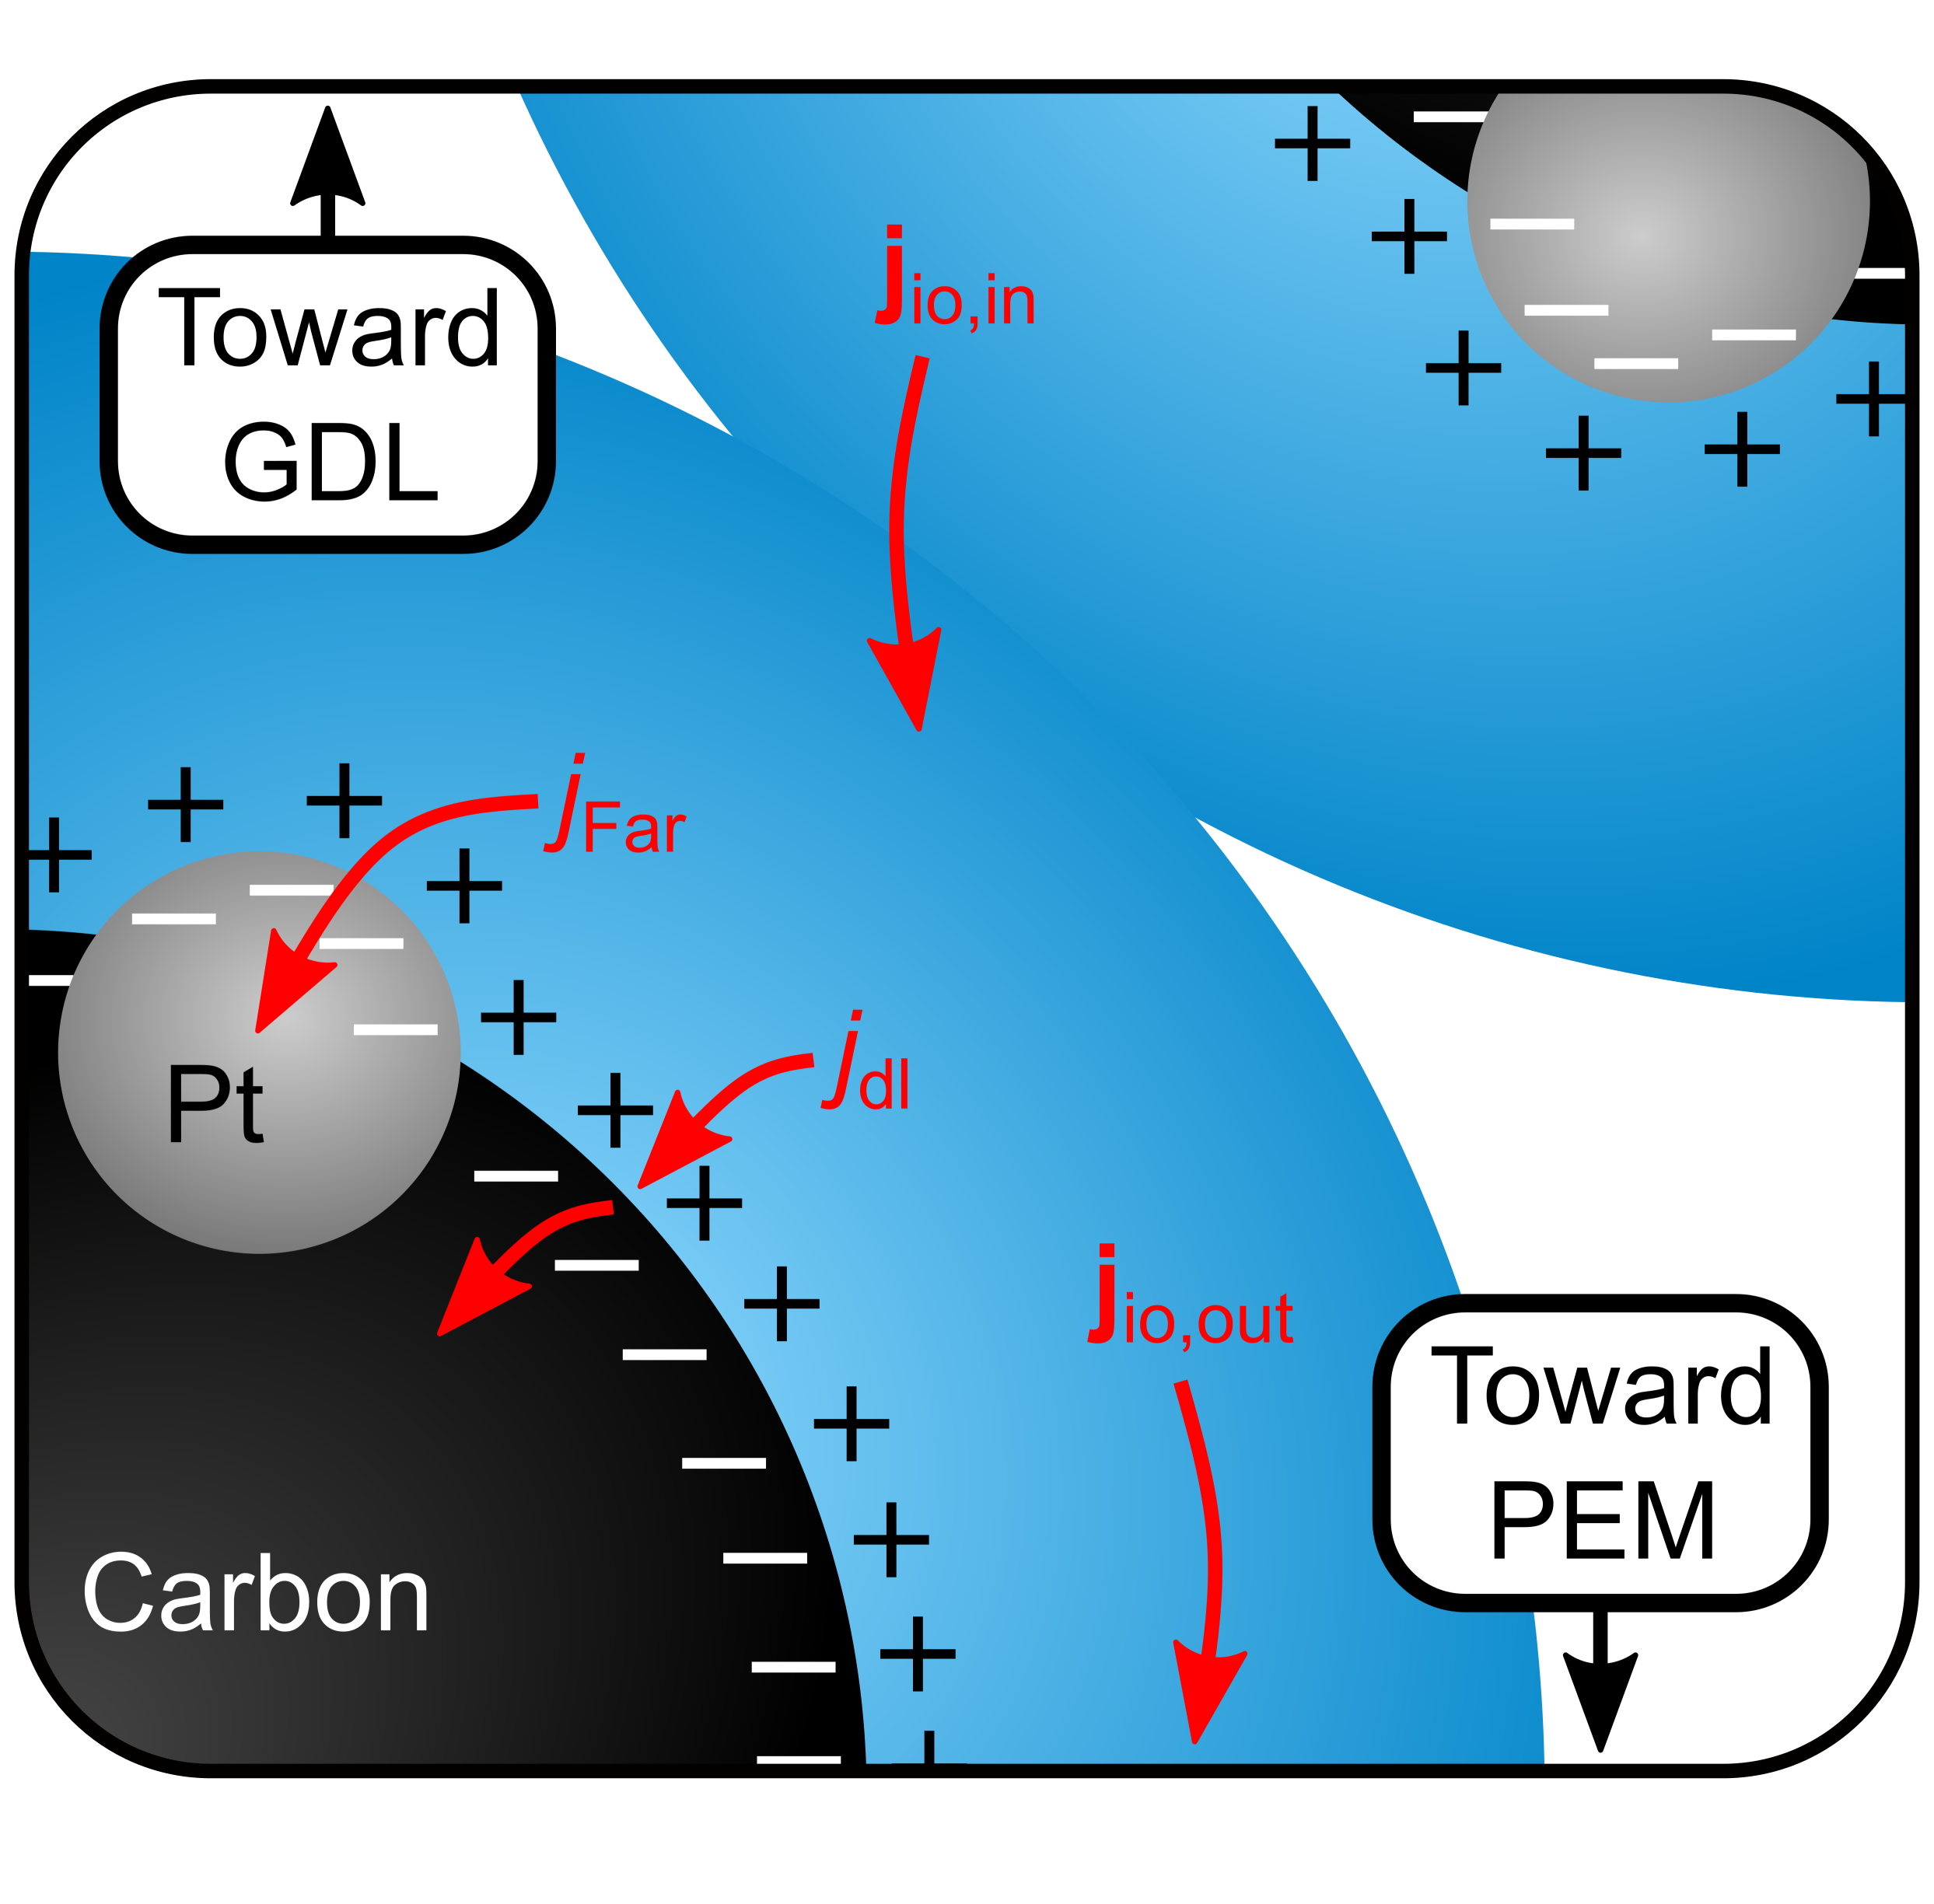
\includegraphics[width=2.487in]{figures/double-layer-2_487in.png}
    \caption{Close up of simulated core-shell particles in the CL. The ionic currents in/out (${\bf j}_{\rm io}$), Faradaic current ($j_{\rm Far}$), and double layer current ($j_{\rm dl}$) that preserve charge within each discretized volume are illustrated to clarify terms in equation~(\ref{eq:double-layer}).}
    \label{fig:double-layer}
\end{figure}

The charge stored in the capacitive double layer provides a differential equation for the evolution of the double layer potential $\Delta\phi_{\rm dl}$:
\begin{equation}
    \frac{d \Delta\phi_{\rm dl}}{d t} = \frac{-j_{\rm dl}}{C_{\rm dl} A_{\rm dl}},
\end{equation}
where $C_{\rm dl}$ and $A_{\rm dl}$ are the specific capacitance (F~m$^{-2}$) and specific double layer area. The double layer potential is defined as the difference between the cathode ($\phi_{\rm ca}$) and Nafion-phase electric potentials,
\begin{equation}
    \Delta\phi_{\rm dl} = \phi_{\rm ca} - \phi_{\rm N}.
\end{equation}
Using the cathode (carbon and Pt) potential as the reference, $\phi_{\rm ca}$ equals zero. Consequently, $\phi_{\rm N}=-\Delta \phi_{\rm dl}$.

\subsection{Surface coverage}

The Pt catalyst surface coverage $\theta_{k, \rm Pt}$ (kmol$_k$~kmol$^{-1}_{\rm tot}$) impacts the oxygen reduction reaction (ORR) kinetics, as discussed in our previous publication~\cite{bib:randall_2020}. Species coverages change in time according to
\begin{equation}
    \frac{d \theta_{k, \rm Pt}}{d t} = \frac{1}{\Gamma} \dot{s}_{k, \rm Pt},
\end{equation}
where $\Gamma$ is the adsorption site density (kmol$_{\rm tot}$~m$^{-2}_{\rm Pt}$). 

\subsection{Reactions and kinetics}
\label{sect:kinetics}

Reactions in the model take place at interfaces between phases. Parentheses are used in the following reactions to denote the host phase for each species. These include gas (g), Nafion (N), liquid (L), Pt surface (s), and cathode carbon phase (ca). Gas-phase oxygen transfers into or out of the Nafion phase
\begin{equation} \label{eq:o2-gn}
    {\rm O_2(g) \leftrightharpoons O_2(N).}
\end{equation}

Water moves between the gas, liquid, and Nafion phases through absorption/desorption and condensation/evaporation reactions
\begin{gather}
    {\rm H_2O(g) \leftrightharpoons H_2O(N),} \label{eq:h2o-gn} \\
    {\rm H_2O(L) \leftrightharpoons H_2O(N),} \label{eq:h2o-wn} \\
    {\rm H_2O(g) \leftrightharpoons H_2O(L).} \label{eq:h2o-gw}
\end{gather}

The ORR is modeled using a two-step mechanism. The first step bonds Nafion-phase oxygen to Pt surface sites: 
\begin{equation} \label{eq:orr-1}
    {\rm O_2(N) + 2Pt(s) \leftrightharpoons 2O(s).} 
\end{equation}
The second step is the charge-transfer reaction, modeled as a single global step:
\begin{equation} \label{eq:orr-2}
    {\rm 2H^{+}(N) + 2e^{-}(ca) + O(s) \leftrightharpoons H_2O(N) + Pt(s).} 
\end{equation}

Excluding reaction~(\ref{eq:orr-2}), concentration dependent reversible mass-action kinetics are used to solve for species production rates. Each reaction $i$ has a net production for species $k$ equal to
\begin{equation} \label{eq:s_dot}
    \dot{s}_{k,i} = \nu_{k,i} \bigg( k_{{\rm fwd},i} \prod_{r} C_{{\rm ac},\,r}^{\nu_{r,i}^{\prime}} 
                  - k_{{\rm rev},i} \prod_{p} C_{{\rm ac},\,p}^{\nu_{p,i}^{\prime \prime}} \bigg), 
\end{equation}
where $k_{{\rm fwd},i}$ and $k_{{\rm rev},i}$ are the forward and reverse rate constants. The reverse rate $k_{{\rm rev},i}$ is calculated based on the forward rate and the equilibrium constant, to ensure thermodynamic reversibility~\cite{bib:decaluwe_weddle_2018}. The forward and reverse stoichiometric coefficients for a species $k$ in reaction $i$ are $\nu_{k,i}^{\prime}$ and $\nu_{k,i}^{\prime \prime}$, respectively. The net stoichiometric coefficients are calculated as $\nu_{k,i} = \nu_{k,i}^{\prime \prime} - \nu_{k,i}^{\prime}$. The products over $r$ and $p$ in equation~(\ref{eq:s_dot}) represent reactants and products, respectively, but are technically over all $k$ species; if a species is not a reactant or product for reaction $i$, then the relevant $\nu_{k,i}$ value is zero.

The Faradaic current $j_{\rm Far}$ (A~m$^{-2}_{\rm Pt}$) for the charge-transfer reaction~(\ref{eq:orr-2}) follows concentration dependent Butler-Volmer kinetics:
\begin{equation}
\begin{split}
    j_{\rm Far} = & j_{\rm o}^{*} 
    \prod_{r} C_{{\rm ac},\,r}^{(1-\beta)\nu_{r}^{\prime}} 
    \prod_{p} C_{{\rm ac},\,p}^{(\beta)\nu_{p}^{\prime \prime}} \\
    & \times \, \Bigg[ \exp \bigg( \frac{-\beta n F \eta}{\Bar{R} T} \bigg) 
        - \exp \bigg( \frac{(1-\beta) n F \eta}{\Bar{R} T} \bigg) \Bigg].
\end{split}
\end{equation}
Here, $\beta$ and $n$ are the symmetry factor and elementary charge transferred to the electron conducting phase in the ORR (i.e., $n = -\nu_{\rm e^{-}}$ in reaction~(\ref{eq:orr-2})). The reference exchange current density ($j_{\rm o}^{*}$) is a rate constant that includes Arrhenius parameters to capture temperature effects. Multiplying $j_{\rm o}^{*}$ by the species activity concentration ($C_{{\rm ac},\,k}$) products provides the exchange current density $j_\circ$. The universal gas constant is $\Bar{R}$, the temperature $T$, the overpotential $\eta$, and Faraday's constant $F$. Net species production rates in reaction~(\ref{eq:orr-2}) are calculated according to Faraday's Law:
\begin{equation}
    \dot{s}_{k,i} = \frac{\nu_{k,i} j_{\rm Far}}{n F}.
\end{equation}

Species activity concentrations are calculated as the activity coefficient multiplied by the species molar concentration for that phase (kmol~m$^{-3}$ for three-dimensional bulk phases, kmol~m$^{-2}$ for surface phases). We assume ideal thermodynamics for this work (activity coefficient equals unity), such that the activity concentrations exactly equal the molar concentrations. All reaction kinetic rate parameters are summarized in table~\ref{tab:kinetics}, and species reference thermodynamics (species enthalpy $h_k^\circ$ and entropy $s_k^\circ$) values at the simulation temperature (i.e. 80$^{\circ}$C) are provided in table~\ref{tab:thermo}.


\begin{table*}[!ht]
    \small
    \centering
    \caption{Kinetic rate constants for all modeled reactions. `Assumed' rate parameters were assumed fast, to keep reactions near equilibrium.}
    \vspace*{1mm}
    
    \begin{tabular}{l c c c c}
    \hline \hline
    Reaction &Rate Constant               &Value         &Units      &Source \\
    \hline \vspace*{-3mm} \\
    (\ref{eq:o2-gn}) \,\, ${\rm O_2(g) \leftrightharpoons O_2(N)}$ &$k_{\rm fwd,\ref{eq:o2-gn}}$   &$2.0$ &m~s$^{-1}$ &assumed\\
    (\ref{eq:h2o-gn}) \,\, ${\rm H_2O(g) \leftrightharpoons H_2O(N)}$ &$k_{\rm fwd,\ref{eq:h2o-gn}}$ &$2.0$ &m~s$^{-1}$ &assumed\\
    (\ref{eq:h2o-wn}) \,\, ${\rm H_2O(L) \leftrightharpoons H_2O(N)}$ &$k_{\rm fwd,\ref{eq:h2o-wn}}$ &$2.0$ &m~s$^{-1}$ &assumed\\
    (\ref{eq:h2o-gw}) \,\, ${\rm H_2O(g) \leftrightharpoons H_2O(L)}$ &$k_{\rm fwd,\ref{eq:h2o-gw}}$ &$2.0$ &m~s$^{-1}$ &assumed\\
    (\ref{eq:orr-1}) \,\, ${\rm O_2(N) + 2Pt(s) \leftrightharpoons 2O(s)}$ & $k_{\rm fwd,\ref{eq:orr-1}}$ &$1.9\times10^{2}$ &m$^5$~mol$^{-2}$~s$^{-1}$ &fit\\
    (\ref{eq:orr-2}) \,\, ${\rm 2H^{+}(N) + 2e^{-}(ca) + O(s) \leftrightharpoons H_2O(N) + Pt(s)}$ &$j_{\rm o}^{*}$ &$\,\,\,\,4.5\times10^{-15}$ &A~m$^{6.5}$~mol$^{-2.5}$ &fit\\
    \hline \hline
    \end{tabular}
    \label{tab:kinetics}
\end{table*}
\begin{table}[!t]
    \small
    \centering
    \caption{Species' reference thermodynamic properties (enthalpies $h^\circ$ and entropies $s^\circ$) at 80$^{\circ}$C. Thicknesses with H$_2$O(N) species correspond to the Nafion thin-films in the NR experiments~\cite{bib:decaluwe_2018}.}
    \vspace*{1mm}
    
    \begin{tabular}{l r r}
    \hline \hline 
    Species            &$h^\circ$ [J~kmol$^{-1}$]     &$s^\circ$ [J~kmol$^{-1}$~K$^{-1}$] \\
    \hline \vspace*{-3mm} \\
    {\bf Gas phase}&&\\
    \hspace{7px}N$_2$(g)           &$1.016\times10^{6}$           &$1.945\times10^{5}$ \\
    \hspace{7px}O$_2$(g)           &$1.027\times10^{6}$           &$2.192\times10^{5}$ \\
    \hspace{7px}H$_2$O(g)          &$-2.406\times10^{8}$          &$2.061\times10^{5}$ \\
    {\bf Liquid water}&& \\
    \hspace{7px}H$_2$O(L)          &$-2.832\times10^{8}$          &$7.825\times10^{4}$ \\
    {\bf Nafion phase}&&\\
    \hspace{7px}H$^{+}$(N)         &$-5.000\times10^{7}$          &$8.677\times10^{2}$ \\
    \hspace{7px}O$_2$(N)           &$2.744\times10^{6}$           &$2.336\times10^{5}$ \\
    \hspace{7px}H$_2$O(N), 5~nm    &$-2.829\times10^{8}$          &$9.826\times10^{4}$ \\
    \hspace{7px}H$_2$O(N), 7~nm    &$-2.830\times10^{8}$          &$9.826\times10^{4}$ \\
    \hspace{7px}H$_2$O(N), 12~nm   &$-2.827\times10^{8}$          &$9.826\times10^{4}$ \\
    \hspace{7px}H$_2$O(N), 18~nm   &$-2.828\times10^{8}$          &$9.826\times10^{4}$ \\
    \hspace{7px}H$_2$O(N), 20~nm   &$-2.828\times10^{8}$          &$9.826\times10^{4}$ \\
    {\bf Pt phase}&&\\
    \hspace{7px}O(s)               &$-1.238\times10^{8}$          &$2.499\times10^{5}$ \\
    \hspace{7px}Pt(s)              &\multicolumn{1}{c}{$0.0$}     &\multicolumn{1}{c}{$\qquad0.0$} \\
    \hline \hline \vspace*{-3mm} 
    \end{tabular}
    \label{tab:thermo}
\end{table}
\subsection{Proton exchange membrane}
\label{sect:pem}

Although the bulk membrane is not explicitly included in the simulation, the drop in potential across this layer ($\Delta \phi_{\rm PEM}$) is approximated by modeling the membrane as a simple resistor:
\begin{equation}
    \Delta \phi_{\rm PEM} = \lvert{\bf j}_{\rm ext}\rvert\, R_{\rm PEM}.
\end{equation}
The external current density (${\bf j}_{\rm ext}$) is a user input to the model. The area specific resistance (ASR) of the membrane ($R_{\rm PEM}$) is taken from Slade et al.~\cite{bib:slade_2002}, using the result measured at the closest temperature and relative humidity to the validation experiments used here~\cite{bib:owejan_2013}, after adjusting to account for membrane thickness.

\subsection{Anode}
\label{sect:anode}

To compare model results to full cell data, the equilibrium potential difference at the PEM-anode interface ($\Delta \phi_{\rm an}^{\rm eq}$) is calculated using the Gibbs free energy for the hydrogen oxidation reaction (HOR), $\Delta g_{\rm HOR}$:
\begin{equation} \label{eq:phi-anode}
    \Delta \phi_{\rm an}^{\rm eq} = \frac{-\Delta g_{\rm HOR}}{n F},
\end{equation}
where the HOR reaction is,
\begin{equation}
    {\rm H_2(N) \leftrightharpoons 2H^{+}(N) + 2e^{-}(an).}
\end{equation}

\subsection{Cell voltage}

The total cell voltage is defined as
\begin{equation}
    V_{\rm cell} = \Delta \phi_{\rm an}^{\rm eq} - \phi_{\rm N,\, int} - \vert{\bf j}_{\rm ext}\rvert\, R_{\rm PEM},
\end{equation}
where $\phi_{\rm N,\, int}$ is the electric potential in the CL Nafion phase at the CL-PEM interface.

\subsection{Boundary conditions}

In the $y$ direction, boundary conditions are imposed at the flow channel and membrane interfaces. For the former, the gas phase in the flow channel is fixed to a constant temperature, density, and composition. Additionally, the flow channel is treated as if it is free of liquid water, i.e. $\epsilon_{\rm w} = 0$. At the CL-PEM interface, zero flux is assumed for the gas and liquid phases:
\begin{equation}
    {\bf J}_{k,\rm g} \big|_{\rm CL-PEM} = {\bf N}_{\rm w} \big|_{\rm CL-PEM} = 0.
\end{equation}
For the proton transport at this same interface, the ionic current into the CL is equivalent to the external current,
\begin{equation} \label{eq:ionic-bc}
    {\bf j}_{\rm io} \big|_{\rm CL-PEM} = -{\bf j}_{\rm ext}.
\end{equation}
Assuming zero electronic current at the PEM interface, equation~(\ref{eq:ionic-bc}) enforces charge neutrality for the entire model domain. Species boundary conditions at the outermost and innermost radii of the Nafion shells at a given depth are defined by the reactions in section~\ref{sect:kinetics}. 


%%%%%%%%%%%%%%%%%%%%%%%%%%%%%%%%%%%%%%%%%%%%%%%%%%%%%%%%%%%%%%%%%%%%%%%%%%
\section{Simulation tools and model accessibility}
In support of open science and research transparency, the model is available as a Github repository~\cite{bib:randall_2021}, as well as all of the files needed to reproduce this manuscipt in its entirety~\cite{bib:pemfc_paper_2021}. The model is written in Python~\cite{bib:python_2022}; any interested party can run, modify, or extend the model under the permissive open source BSD 3-clause license. Directions for setting up a suitable environment within Python are included in the repository README .

\subsection{Numerical integrator}
The set of differential equations described above is integrated with the SciPy `solve\_ivp' routine, using the implicit `BDF' method~\cite{bib:scipy_2022}. We define a Jacobian pattern, which is provided to the solver to improve computational efficiency. A simulation time of $1 \times 10^6$~seconds ensures steady-state is reached at the open circuit condition. Afterward, the steady-state condition is saved and reused to initialize the state variables for the first user-defined current density. For each subsequent current density, the steady-state solution from the previous current density is used as the initial condition, which reduces the simulation time needed to reach steady state to less than 100~s (and typically much less than this). Implementing these computational efficiencies, a polarization curve is generated in roughly two minutes. 

\subsection{Cantera}
The open-source Cantera library handles the gas-phase transport parameters, species thermodynamics, and reaction kinetics~\cite{bib:cantera_2017}. Cantera includes routines for common phase models (e.g., ideal gas) that provide diffusion coefficients, molecular weights, partial pressures, and viscosities. Cantera also handles the chemical and charge-transfer kinetic calculations, as in section~\ref{sect:kinetics}. Use of Cantera allows a generalized code structure where important details are set entirely in the input file, rather than in the model codebase.


%%%%%%%%%%%%%%%%%%%%%%%%%%%%%%%%%%%%%%%%%%%%%%%%%%%%%%%%%%%%%%%%%%%%%%%%%%
\section{Structure-property relationships}
\label{sect:struct-prop-relationships}

\begin{figure*}[htb!]
    \centering
    
\includegraphics[width=5.008in]{figures/Nafion-structure-5_008in.png}
    \caption{Illustration of hypothesized structures at carbon-Nafion and Pt-Nafion interfaces. The (a) uniform method assumes a homogeneous thin film with reduced water uptake compared to bulk Nafion. The (b) mixed method instead assumes interfacial water-rich and water-poor regions near the Pt while the carbon interfaces maintain a uniform composition.}
    \label{fig:struct-models}
\end{figure*}

The equations in section~\ref{sect:model-framework} are common throughout PEMFC modeling~\cite{bib:weber_2004, bib:weber_2014, bib:arif_2020}, and are extended here with novel structure-property relationships to predict CL transport parameters (e.g. $D_{k,\rm N}^{\rm av}, \ \sigma_{\rm io}$). These parameters are not well known for nano-thin Nafion films. Thus far models have commonly used $D_{k,\rm N}^{\rm av}$ and $\sigma_{\rm io}$ values measured from bulk Nafion membranes~\cite{bib:springer_1991, bib:weber_2004, bib:chu_2003, bib:ismail_2017, bib:aghighi_2017}. Literature over the last decade, however, has shown that transport through nano-thin Nafion films departs significantly from bulk membrane behavior~\cite{bib:decaluwe_2018, bib:paul_mccreery_2014, bib:paul_2014}, due to reduced water uptake and confinement effects near substrate interfaces~\cite{bib:dura_2009, bib:decaluwe_2018, bib:kusoglu_2012, bib:kusoglu_2017}.

In our previous publication~\cite{bib:randall_2020}, we incorporated accurate transport parameters in a PEMFC model using structure-property relationships developed specifically for thin film Nafion. These relationships combined quantitative structural data from neutron reflectometry (NR) experiments~\cite{bib:decaluwe_2018} with separate conductivity measurements~\cite{bib:paul_mccreery_2014} -- both performed using nano-thin Nafion films. In this previous work, Nafion-phase water was assumed constant, equilibrated with a constant relative humidity gas phase. In this work, we allow the gas- and Nafion-phase water content to vary (and allow for liquid water condensation and evaporation), and have updated these relationships to depend upon varying local ionomer water content. This process is detailed below.

\subsection{Nafion-phase water}

In DeCaluwe et al.~\cite{bib:decaluwe_2018}, the maximum possible water uptake in thin-film Nafion at a given relative humidity correlates with film thickness in a non-monotonic manner. One goal of the present work is to understand the relationship between ionomer loading and limiting phenomena in PEMFCs. Here, we describe the Nafion-phase water thermodynamic calculations. The reference thermodynamic properties for a species $k$ (enthalpy $h_k^\circ$, entropy $s_k^\circ$, and Gibbs free energy $g_k^\circ$) are calculated using the seven-coefficient NASA polynomial~\cite{bib:mcbride_1993}. For each Nafion film thickness simulated, we used SciPy's `optimize' routine to find the thermodynamic coefficients that result in the correct equilibrium Nafion water volume fraction, according to the NR experiments~\cite{bib:decaluwe_2018}.
% As an example, the reference enthalpy ($h^0(T)$) of liquid water is calculated using 
%\begin{equation}
%\begin{split}
%    h^0(T) = \Bar{R} \bigg( a_0 T + \frac{a_1}{2} T^2 + \frac{a_2}{3} T^3 \\
%           + \frac{a_3}{4} T^4 + \frac{a_4}{5} T^5 + a_5 \bigg),
%\end{split}
%\end{equation}
%where the $a_i$ values are defined coefficients.
% To build the Nafion-phase water species, this same thermodynamic model was used. The given coefficients for pure liquid water were kept the same, with the exception of $a_5$. A new value for $a_5$ shifts the reference enthalpy without any impact to the reference entropy. Rather than arbitrarily picking a new coefficient for this species, an optimization routine was performed. First, the Nafion-phase object was constructed in python with the composition set so that the steady-state water volume fraction matched that of the experiments performed in~\cite{bib:decaluwe_2018}. Afterward, a simulated gas phase object that also matched the relative humidity and temperature from this study was created. Finally, using SciPy.optimize, a new $a_5$ coefficient was determined by minimizing any additional absorption/desorption between the gas and Nafion phases. This process was repeated for each relevant Nafion thickness from the study (i.e. 5~nm, 7~nm, 12~nm, 18~nm, and 20~nm), saving each respective new coefficient.
When non-uniform ionomer loadings are modeled, the appropriate coefficients are used to calculate the local Nafion-phase water thermodynamics, as a function of local dry Nafion thickness. 

\subsection{Thin film structural approximations}

The NR and conductivity measurements used to develop the structure-property relationships were performed with Nafion on silicon substrates. In a PEMFC CL, Nafion binds to carbon and Pt rather than silicon. Others have studied Nafion on Pt and carbon~\cite{bib:wood_2009, bib:shrivastava_2018, bib:dura_2009, bib:ito_2020}, but fewer details are included, providing no clear path to capture transport property variations with varying Nafion thickness. Instead, we propose two hypothetical structural approximations, illustrated in figure~\ref{fig:struct-models}. These approximations are informed by studies showing that Nafion at Pt and carbon interfaces tends to have less structure than at silicon interfaces~\cite{bib:wood_2009, bib:ito_2020, bib:dura_2009, bib:shrivastava_2018}. In some cases, the Nafion structure is homogeneous (i.e. the water uptake is uniformly distributed throughout the film). This is more likely to occur at carbon-Nafion interfaces due to carbon being more hydrophobic and rougher than silicon. The `uniform' method in figure~\ref{fig:struct-models}(a) considers the Nafion ionomer to be uniform, with water uptake equal to that measured by NR for similarly thin films. The structure in the `mixed' model (figure~\ref{fig:struct-models}(b)) includes alternating interfacial layers of water-rich and water-poor Nafion at the Pt-Nafion interfaces and uniform water uptake at the carbon-Nafion interfaces. This method is consistent with reported structures observed at Pt-Nafion interfaces~\cite{bib:wood_2009, bib:dura_2009, bib:shrivastava_2018}. For the remainder of this publication these methods are referred to as `uniform' and `mixed'.

\subsection{Ionic conductivity}
\label{sect:ionic-conductivity}

For bulk Nafion membranes, the ionic conductivity is described empirically by~\cite{bib:springer_1991}:
\begin{equation} \label{eq:sigma-bulk}
\begin{split}
    \sigma_{\rm io, bulk}(\lambda,T) = (0.5139\lambda - 0.326) \\
                                     \times \exp \bigg( 1268 \bigg( \frac{1}{303} 
                                     - \frac{1}{T} \bigg) \bigg),
\end{split}
\end{equation}
which captures the impacts of water uptake $\lambda$ and temperature $T$. In the `uniform' structural method, we use the radially averaged water uptake ($\lambda_{\rm av}$) from the model and a scaling factor ($f_{\rm uniform}$) to get 
\begin{equation} \label{eq:sigma-uniform}
    \sigma_{\rm io, uniform} = \sigma_{\rm io, bulk}(\lambda_{\rm av},T) f_{\rm uniform}.
\end{equation}
The scaling factor is calculated in~\cite{bib:decaluwe_2018} for the thicker uniform Nafion layer present at the gas interface

When the `mixed' method is used, the conductivity at the Pt interface is assumed to be the same as that measured at a silicon interface. Interpolation of the data in~\cite{bib:paul_mccreery_2014} provides the Nafion conductivity near the Pt interfaces ($\sigma_{\rm io, Pt-N}$). This accounts for temperature, water uptake, and thickness dependence. Afterward, the mixed conductivity is calculated using a parallel circuit analogy: 
\begin{equation}
    \sigma_{\rm io, mixed} = 
    \frac{A_{\rm Pt-N}\,\sigma_{\rm io, Pt-N} + A_{\rm C-N}\,\sigma_{\rm io, uniform}}{A_{\rm Pt-N}+A_{\rm C-N}},
\end{equation}
where $A_{\rm Pt-N}$ and $A_{\rm C-N}$ are the areas of the Pt-Nafion and carbon-Nafion interfaces for a single representative core-shell particle, respectively.

\subsection{Oxygen diffusion}

A similar procedure was used to calculate local oxygen diffusion coefficients. The empirical relationship for bulk Nafion is taken from~\cite{bib:sethuraman_2009},
\begin{equation}
    D_{\rm O2, bulk}(T) = 1.745 \times 10^{-9} \exp \bigg( \frac{-1514}{T} \bigg).
\end{equation}
To add water uptake -- and thus thickness -- dependence, the bulk value is scaled linearly by the local $\lambda_{\rm av}$ value at any given time. This assumes that oxygen diffuses through the water domains in the Nafion, and that the mobility therefore decreases linearly with the water content. Further, we assume that the scaling factor ($f_{\rm uniform}$) in equation~(\ref{eq:sigma-uniform}) represents a general decrease in Nafion species' mobilities, and calculate $D_{\rm O2, N}^{\rm av}$ as:
\begin{equation}
    D_{\rm O2, uniform}^{\rm av} = D_{\rm O2, bulk}(T) \frac{\lambda_{\rm av}}{\lambda_{\rm ref}} f_{\rm uniform},
\end{equation}
where the reference $\lambda_{\rm ref}$ is that for a bulk Nafion membrane at the same temperature and RH.

For the mixed method, the layer thicknesses and water uptakes from the silicon-Nafion NR data were used to approximate the interfacial diffusion coefficients,
\begin{equation}
    D_{{\rm O2},i} = D_{\rm O2, bulk}(T) \frac{\lambda_{i}}{\lambda_{\rm ref}} f_{i}.
\end{equation}
The total average diffusion coefficient was then determined by a thickness-weighted average of the layers in series
\begin{equation}
    D_{\rm O2, mixed}^{\rm av} = \frac{\sum t_i}{\sum t_i / D_{{\rm O2},i}},
\end{equation}
where $t_i$ is the thickness of layer $i$, as previously measured~\cite{bib:decaluwe_2018}. Because the oxygen concentration gradients occur locally near the Pt catalysts, a weighting based on Pt-Nafion and carbon-Nafion areas was not used for $D_{\rm O2, N}^{\rm av}$. Instead, the `mixed' approach assumes that all of the Nafion-phase oxygen moves through the interfacial layers located near the Pt catalyst.

%%%%%%%%%%%%%%%%%%%%%%%%%%%%%%%%%%%%%%%%%%%%%%%%%%%%%%%%%%%%%%%%%%%%%%%%%%
\section{Results and Discussion}

\subsection{Model validation}

Simulations were run with pressure and temperature inputs of 150~kPa and 80$^{\circ}$C, respectively. These conditions match the validation experiments from Owejan et al.~\cite{bib:owejan_2013}. Experiments included PEMFCs with four Pt loadings between 0.025 and 0.2~mg$_{\rm Pt}$~cm$^{-2}$. All geometric and transport parameters were adapted from experiments and literature, and were not varied during validation/fitting. Rather, the two kinetic rate constants for the two-step ORR mechanism were adjusted by hand until a minimum goodness-of-fit statistic (see section~\ref{sec:structure_prop_results}) was achieved across all four data sets; the values are reported in table~\ref{tab:kinetics}. Experimental tests using both air and pure oxygen in the cathode gas channel were fit. Figure~\ref{fig:validation_air} shows the model results plotted against the air data set. Comparison to the oxygen data set is available in figure~\ref{fig:validation_o2}.

\subsubsection{Resolving structure-property relationships}
\label{sec:structure_prop_results}

In figure~\ref{fig:validation_air}, $\chi^2$ is used as a goodness-of-fit statistic. It is calculated as
\begin{equation}
    \chi^2 = \frac{1}{n_{\rm pts}} \sum_{i=1}^{n_{\rm pts}} 
             \frac{(V_{i,\rm mod} - V_{i,\rm dat})^2}{{\rm SD}_{i,\rm dat}^2},
\end{equation}
where $n_{\rm pts}$ is the number of experimental data points. For each data point $i$ corresponding to a measured current density, $V_{i,\rm mod}$ is the voltage calculated in the model at that current density, $V_{i,\rm dat}$ is the experimentally measured voltage, and ${\rm SD}_{i,\rm dat}$ is the standard deviation of the data from the mean, taken from error bars reported with the data. A lower $\chi^2$ signifies a better fit, $\chi^2 = 1.0$ is an ideal fit, and $\chi^2 < 1.0$ implies over-fitting. As a rule-of-thumb, $\chi^2 < 2.0$ indicates a good fit to the data. 

\begin{figure}[!tb]
    \centering
    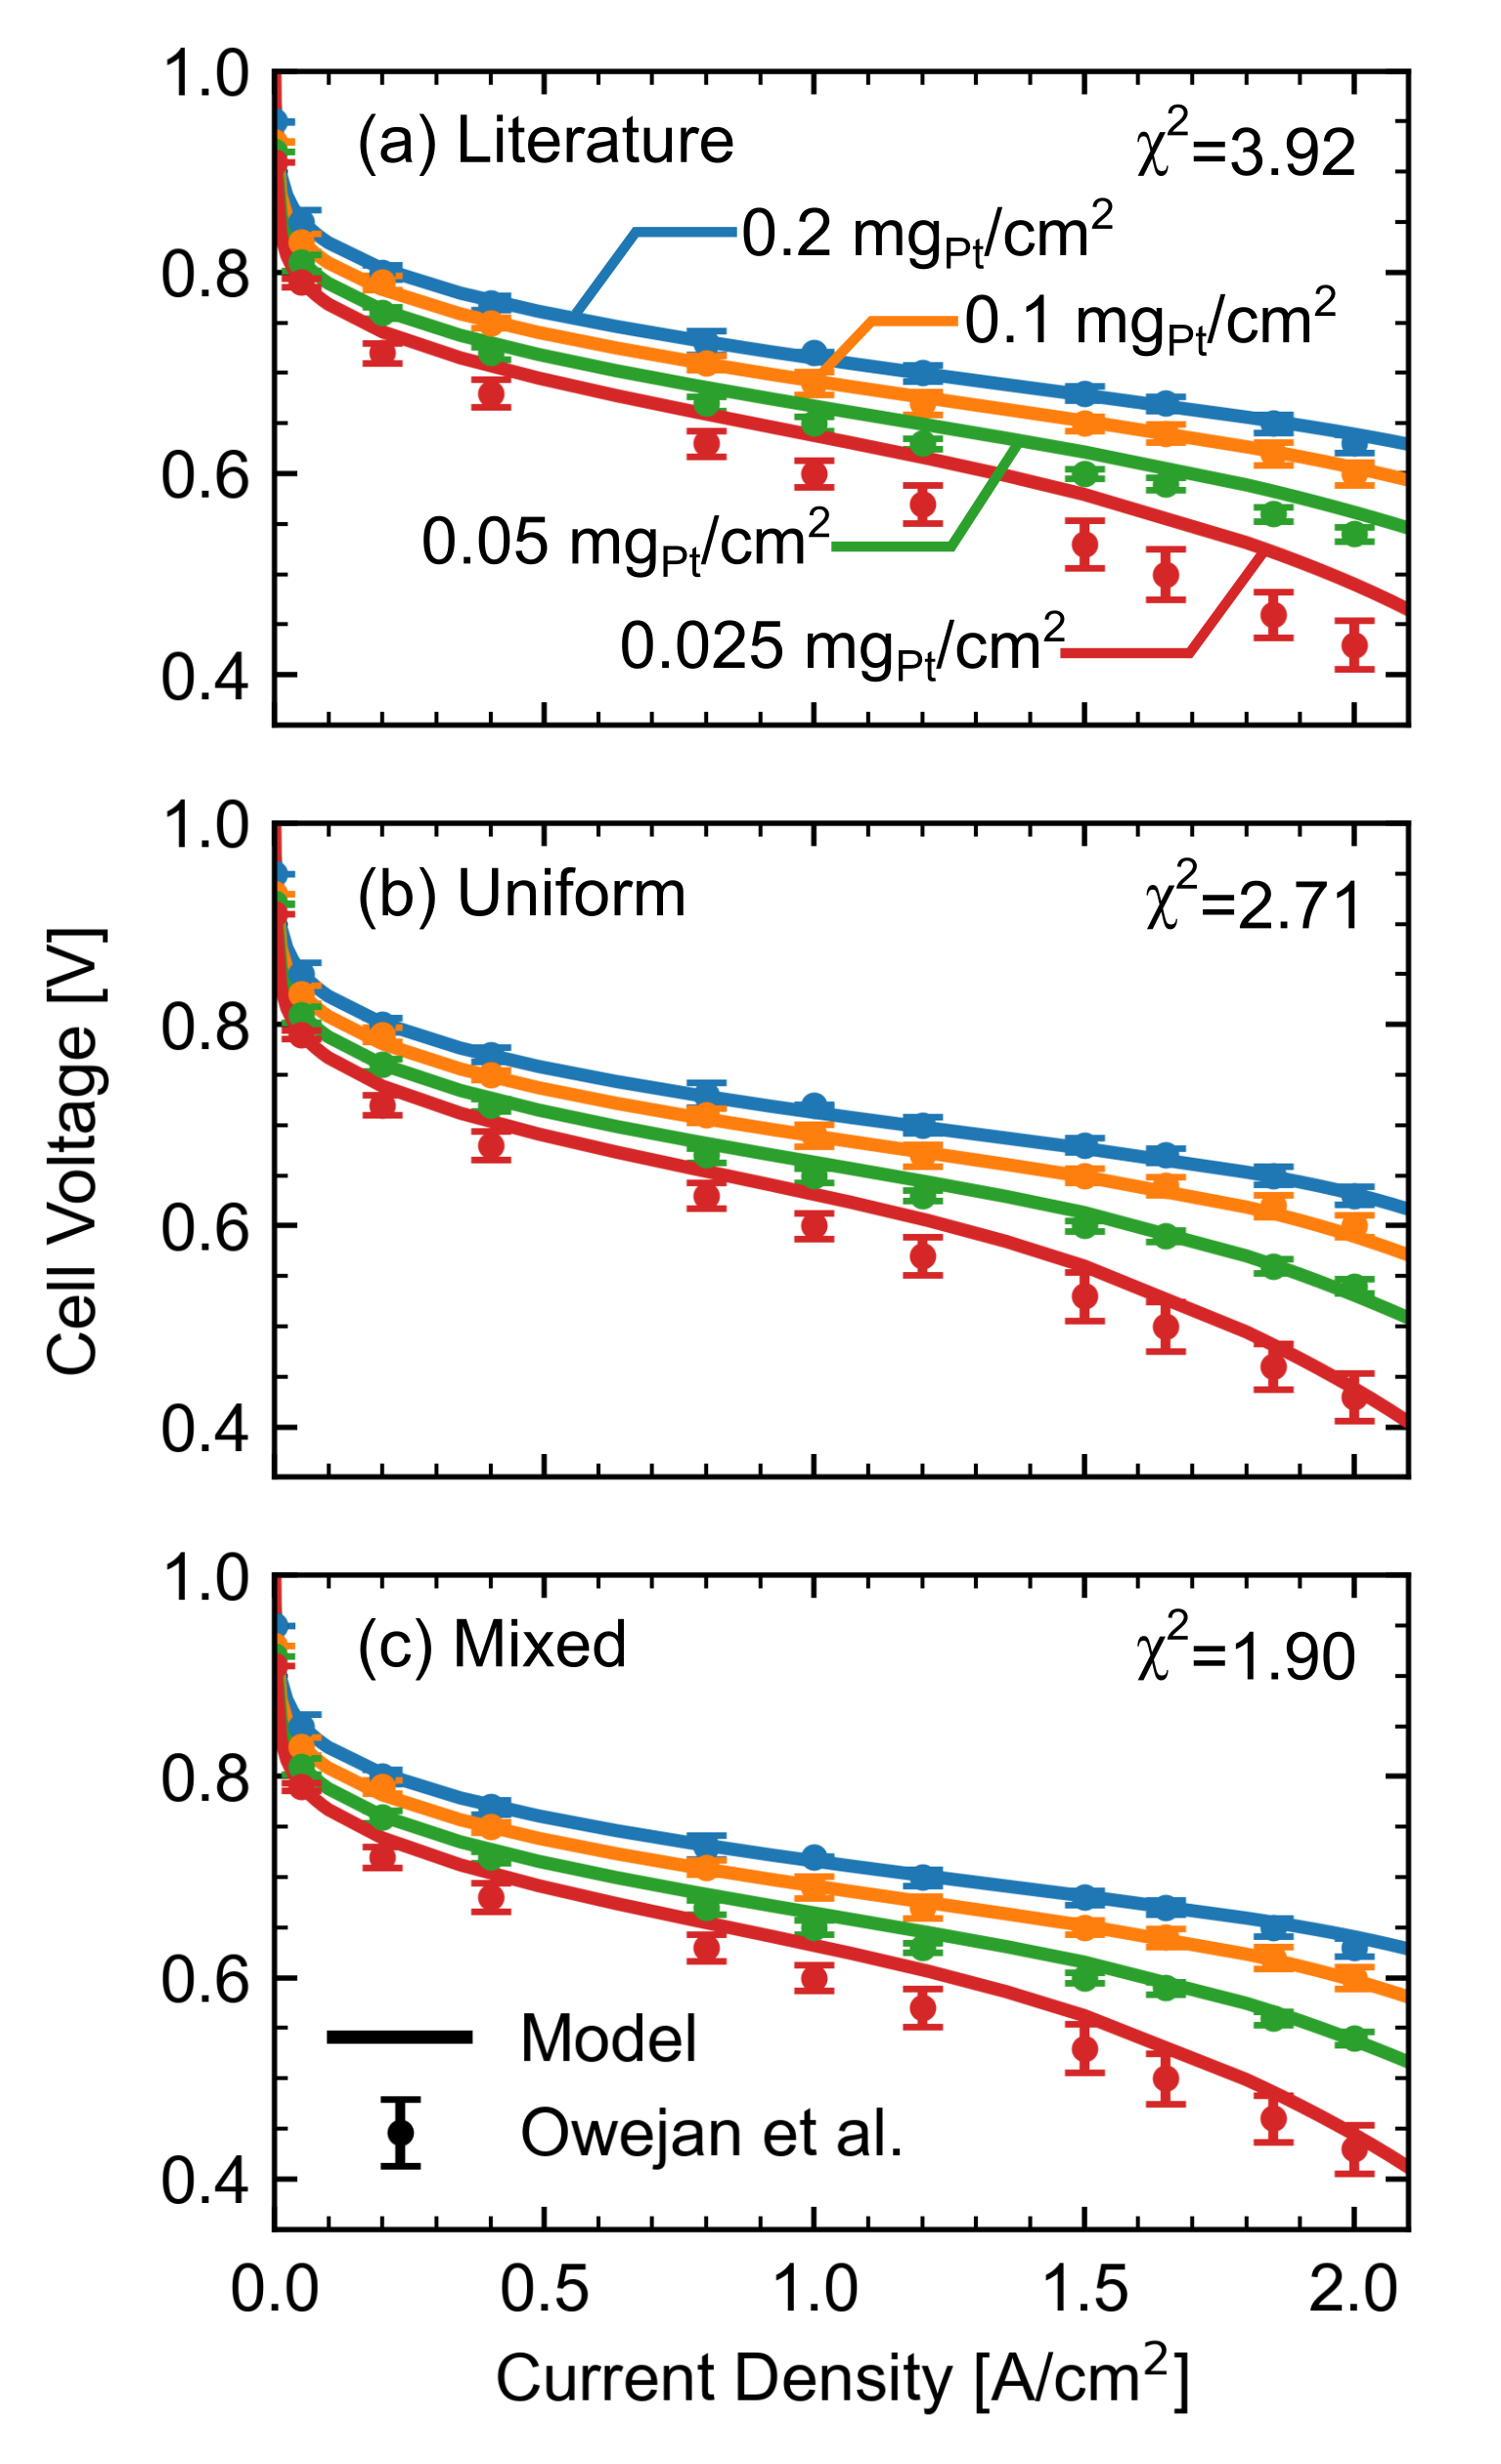
\includegraphics[width=3.07in]{figures/validation-air-vert-3_07in.png}
    \caption{Simulation results and experimental data~\cite{bib:owejan_2013} for air-fed PEMFCs with varying Pt loading. Transport properties within thin-film Nafion are taken from (a) literature~\cite{bib:yadav_2012, bib:sethuraman_2009} and (b-c) structure-property relationships developed within this work. Differences between the (b) uniform and (c) mixed structure-property relationships are described in section~\ref{sect:struct-prop-relationships}.}
    \label{fig:validation_air}
\end{figure}

The three sets of polarization curves in figure~\ref{fig:validation_air} show the best model fits for three different sets of thin-film Nafion transport parameters. In (a), the ionic conductivity and oxygen diffusion coefficient are assumed to be the same as a bulk membrane and are taken from literature~\cite{bib:yadav_2012, bib:sethuraman_2009}. Although the model matches the data at 0.1 and 0.2~mg$_{\rm Pt}$~cm$^{-2}$, it fits poorly at lower Pt loadings. In comparison, (b) and (c) use the `uniform' and `mixed' structure-property relationships discussed in section~\ref{sect:struct-prop-relationships}. These transport parameters provide a significant improvement to the fit at low Pt loadings, while still matching performance at higher loadings. Although the fits in figures~\ref{fig:validation_air}(b) and~(c) are visually indistinguishable, the $\chi^2$ metric implies that the `mixed' transport property method provides a superior fit.

\subsubsection{Losses with low Pt loading}
\label{sect:cause-of-losses}

Exploring the spatial distribution of state and process variables helps identify limiting behaviors at low Pt loading. Figure~\ref{fig:cause-of-losses} shows the distribution of the water saturation, Nafion-phase oxygen density ($\rho_{\rm O2,N}$) at the Pt-Nafion interface, and Faradaic current (normalized to the total external current) for the `mixed' transport model. These are plotted for the highest and lowest Pt loadings (0.2 and 0.025~mg$_{\rm Pt}$~cm$^{-2}$, respectively) at an external current density ${\bf j}_{\rm ext} = 2.0$~A~cm$^{-2}$, where we see the greatest Pt loading effects. In (a), water saturation decreases and associated flooding limitations are less severe at lower Pt loading. The Nafion-phase oxygen density for the innermost radial node is higher for the lower Pt loading, as shown in (b). This suggests that oxygen diffusion through the Nafion shells is not limiting at this current, and does not \emph{directly} explain the performance losses at low Pt loading. 

\begin{figure}[!tb]
    \centering
    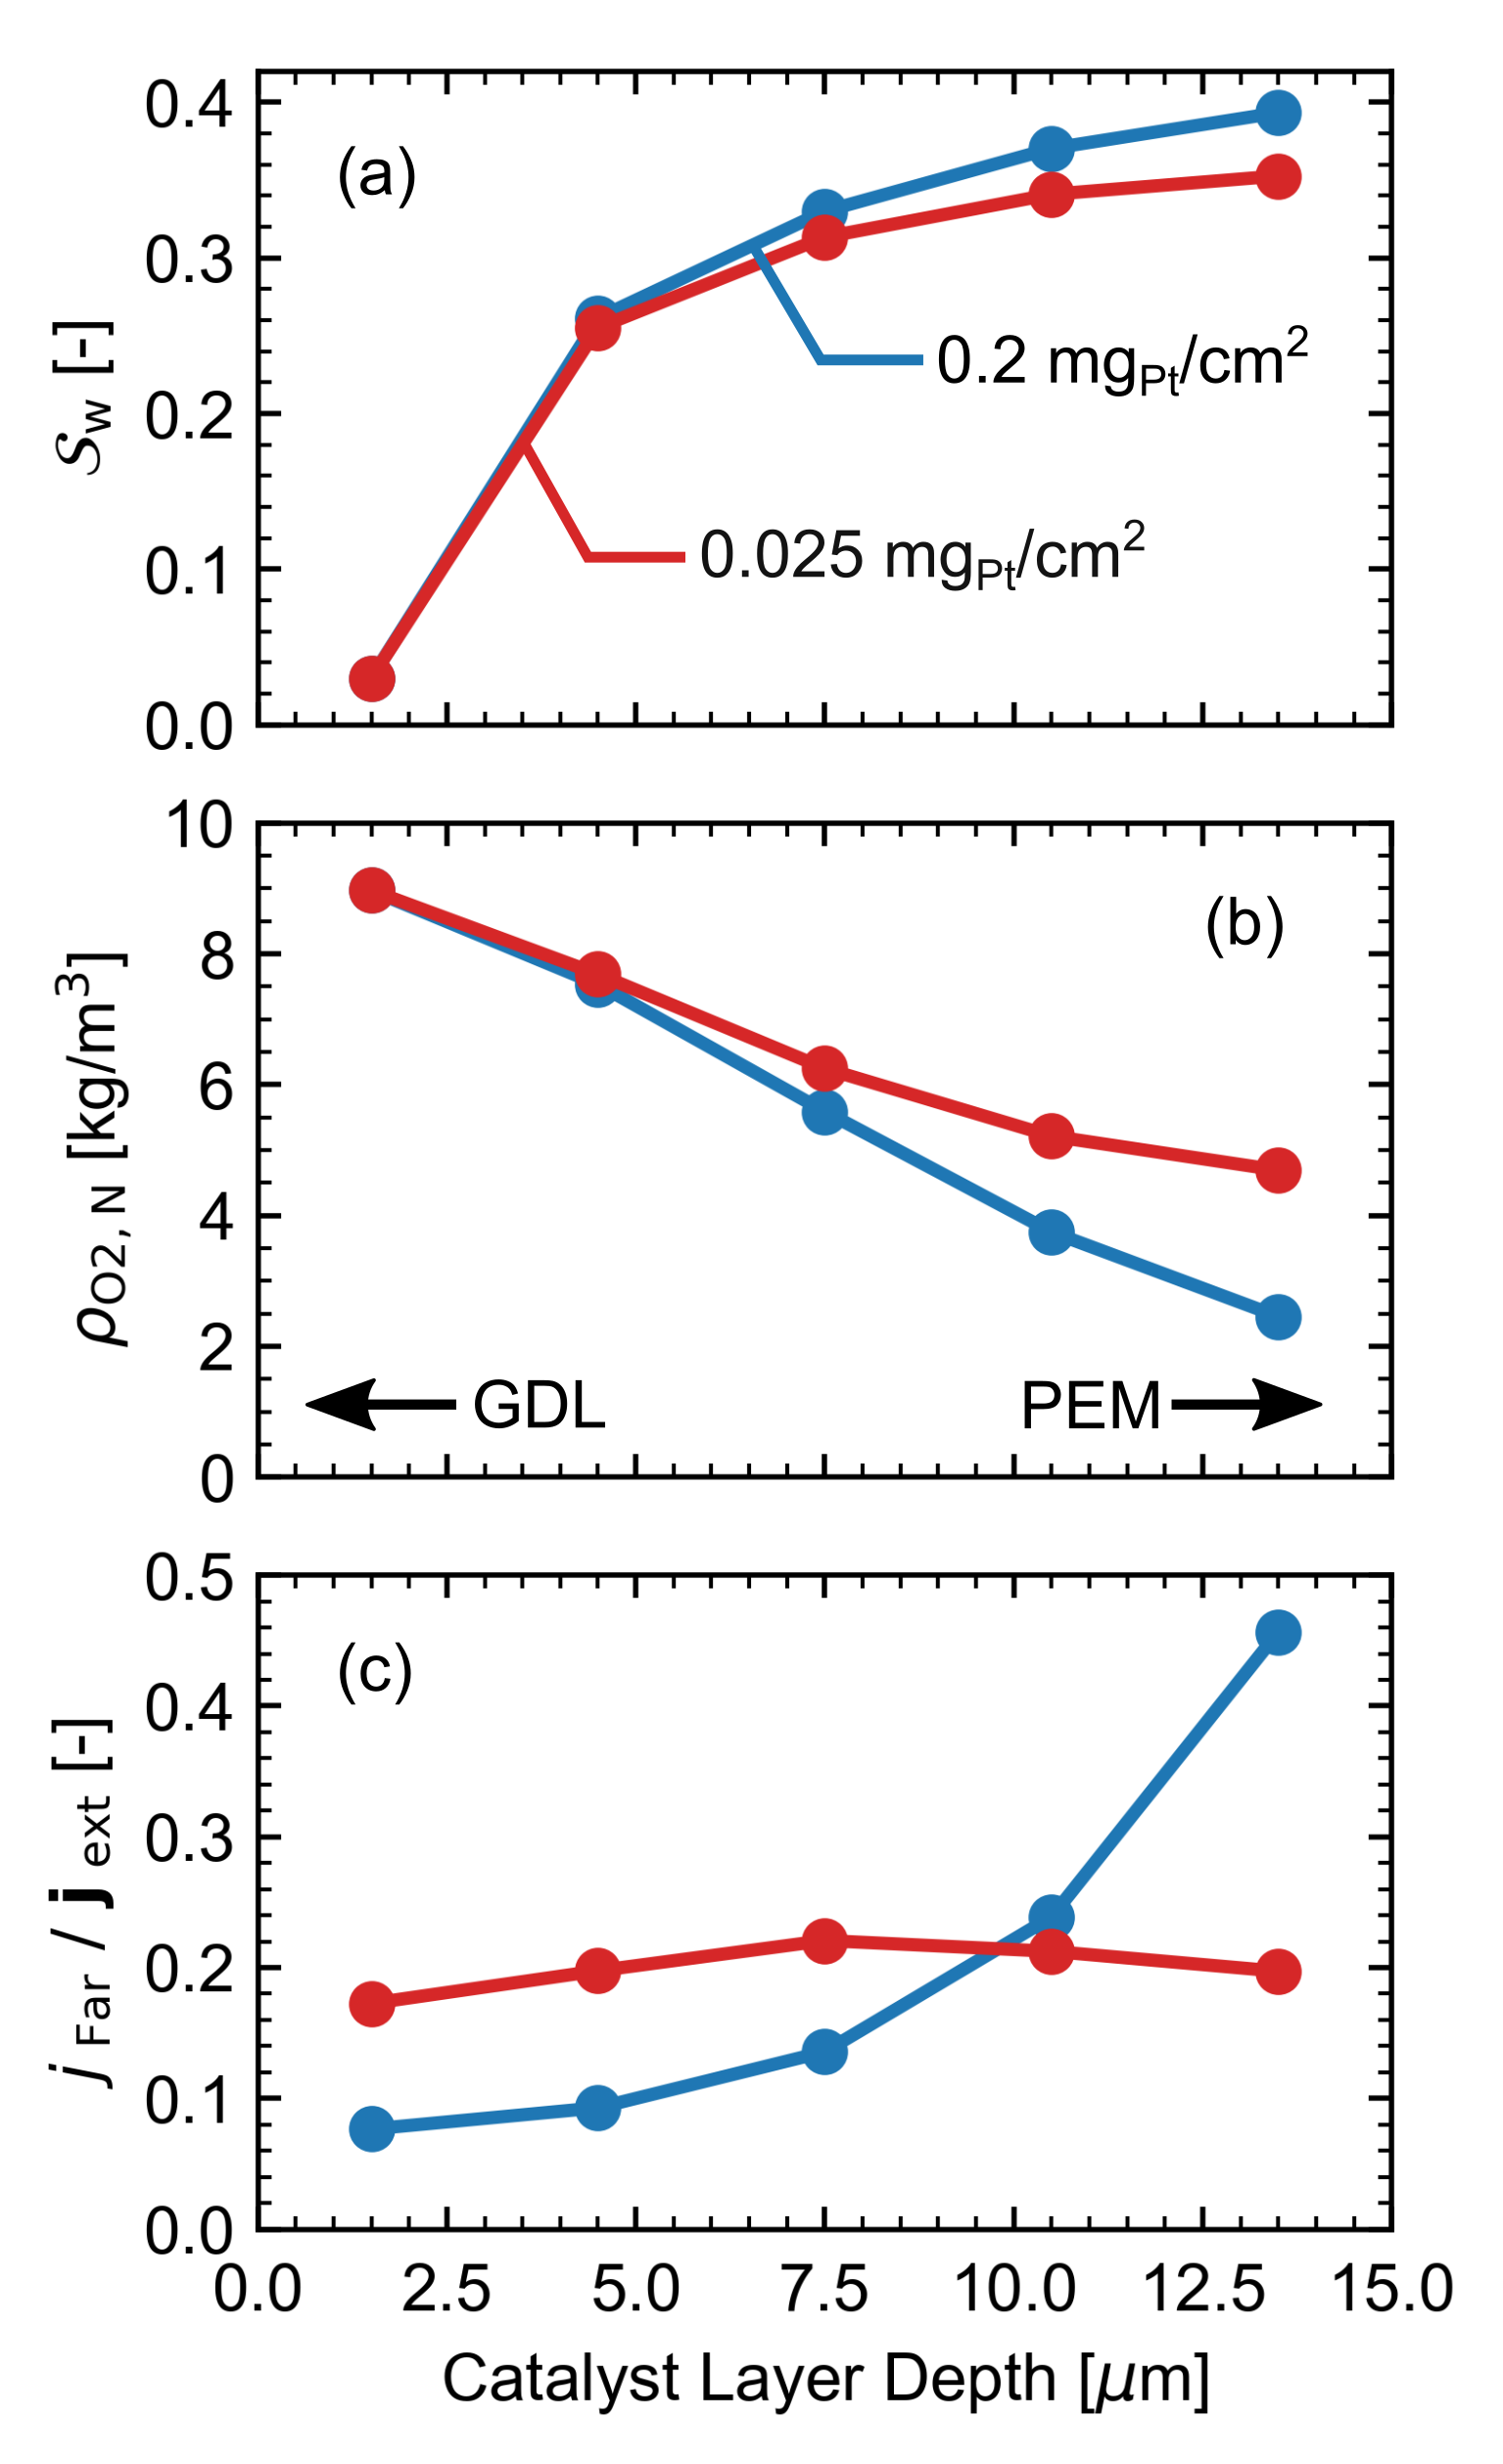
\includegraphics[width=3.07in]{figures/cause-of-losses-vert-3_07in.png}
    \caption{Depth profiles for (a) water saturation, (b) Nafion-phase oxygen density (for the innermost shell), and (c) Faradaic current distributions (normalized by ${\bf j}_{\rm ext}$) within the CL at a current density of 2.0~A~cm$^{-2}$. Plots are oriented with the GDL interface at the left and the PEM interface at the right. Only the highest and lowest Pt loading results are shown from the simulations using the `mixed' transport method.}
    \label{fig:cause-of-losses}
\end{figure}

Rather, the difference between $\rho_{\rm O2,N}$ for the two Pt loadings suggests that differences in the distribution of charge-transfer reactions throughout the CL are key to understanding Pt loading effects. The difference between the two loadings is largest closest to the membrane, suggesting that the O$_2$ flux through the Nafion, and therefore the local Faradaic current, is concentrated in regions near the membrane at high Pt loading, but not at low Pt loading. This is confirmed in figure~\ref{fig:cause-of-losses}(c), which shows the fraction of the total Faradaic current occurring at each CL depth. With higher Pt loadings, there is enough Pt in regions close to the membrane to support most of the required Faradaic current densities, even at high currents. Consequently, we see that nearly 50\% of the charge-transfer reactions occur in the volume adjacent to the membrane, at 0.2~mg$_{\rm Pt}$~cm$^{-2}$. At the lower loading of 0.025~mg$_{\rm Pt}$~cm$^{-2}$, higher activation overpotentials would be required to produce this same Faradaic current in this same volume. The relatively uniform distribution of the Faradaic current throughout the CL at low Pt loading shows that the PEMFC losses are reduced by moving the protons further into the CL to access additional Pt surface located there. The even Faradaic current distribution also helps explain the results in (a) and (b). If ORR occurs evenly throughout the CL, then O$_{2}$(N) depletion and the build-up of liquid water deep into the CL will both be less severe.

These results suggest that, rather than increased activation overpotentials, performance losses at lower Pt loadings instead result directly from larger \emph{Ohmic} losses. To test this theory, figure~\ref{fig:effective-Ohmic-measures} plots the effective Ohmic overpotential ($\eta_{\rm Ohm}^{\rm eff}$) and Ohmic resistance ($R_{\rm Ohm}^{\rm eff}$) associated with CL ion conduction. The effective Ohmic overpotential is calculated as:
\begin{equation}
    \eta_{\rm Ohm}^{\rm eff} = \sum_{i=1}^{N_{y}} \frac{|{\bf j}_{{\rm io},i}|}{\sigma_{{\rm io},i}}
                          \frac{|{\bf j}_{{\rm io},i}|}{|{\bf j}_{\rm ext}|} \Delta y_i,
\end{equation}
where $N_y$ is the number of $y$ nodes in the CL. $\sigma_{{\rm io},i}$ and $\Delta y_{i}$ are the local conductivity and thickness in the $y$-direction for node $i$ (where $\sigma_{{\rm io},i}$ depends on the local Nafion thickness and current water uptake $\lambda$, as in section~\ref{sect:struct-prop-relationships}). The ionic current that passes through each node (${\bf j}_{{\rm io},i}$) is equal to
\begin{equation} \label{eq:eta-ohm-eff}
    {\bf j}_{{\rm io},i} = {\bf j}_{\rm ext} - \sum_i j_{{\rm Far},i} A_{\rm Pt} \Delta y, 
\end{equation}
where $i=1$ corresponds to the CL-PEM interface. Therefore ${\bf j}_{{\rm io},i}$ decreases as we move further into the CL ($i$ increases). The effective Ohmic resistance is defined as:
\begin{equation} \label{eq:R-ohm-eff}
    R_{\rm Ohm}^{\rm eff} = \frac{\eta_{\rm Ohm}^{\rm eff}}{|{\bf j}_{\rm ext}|}.
\end{equation}

\begin{figure}[!tb]
    \centering
    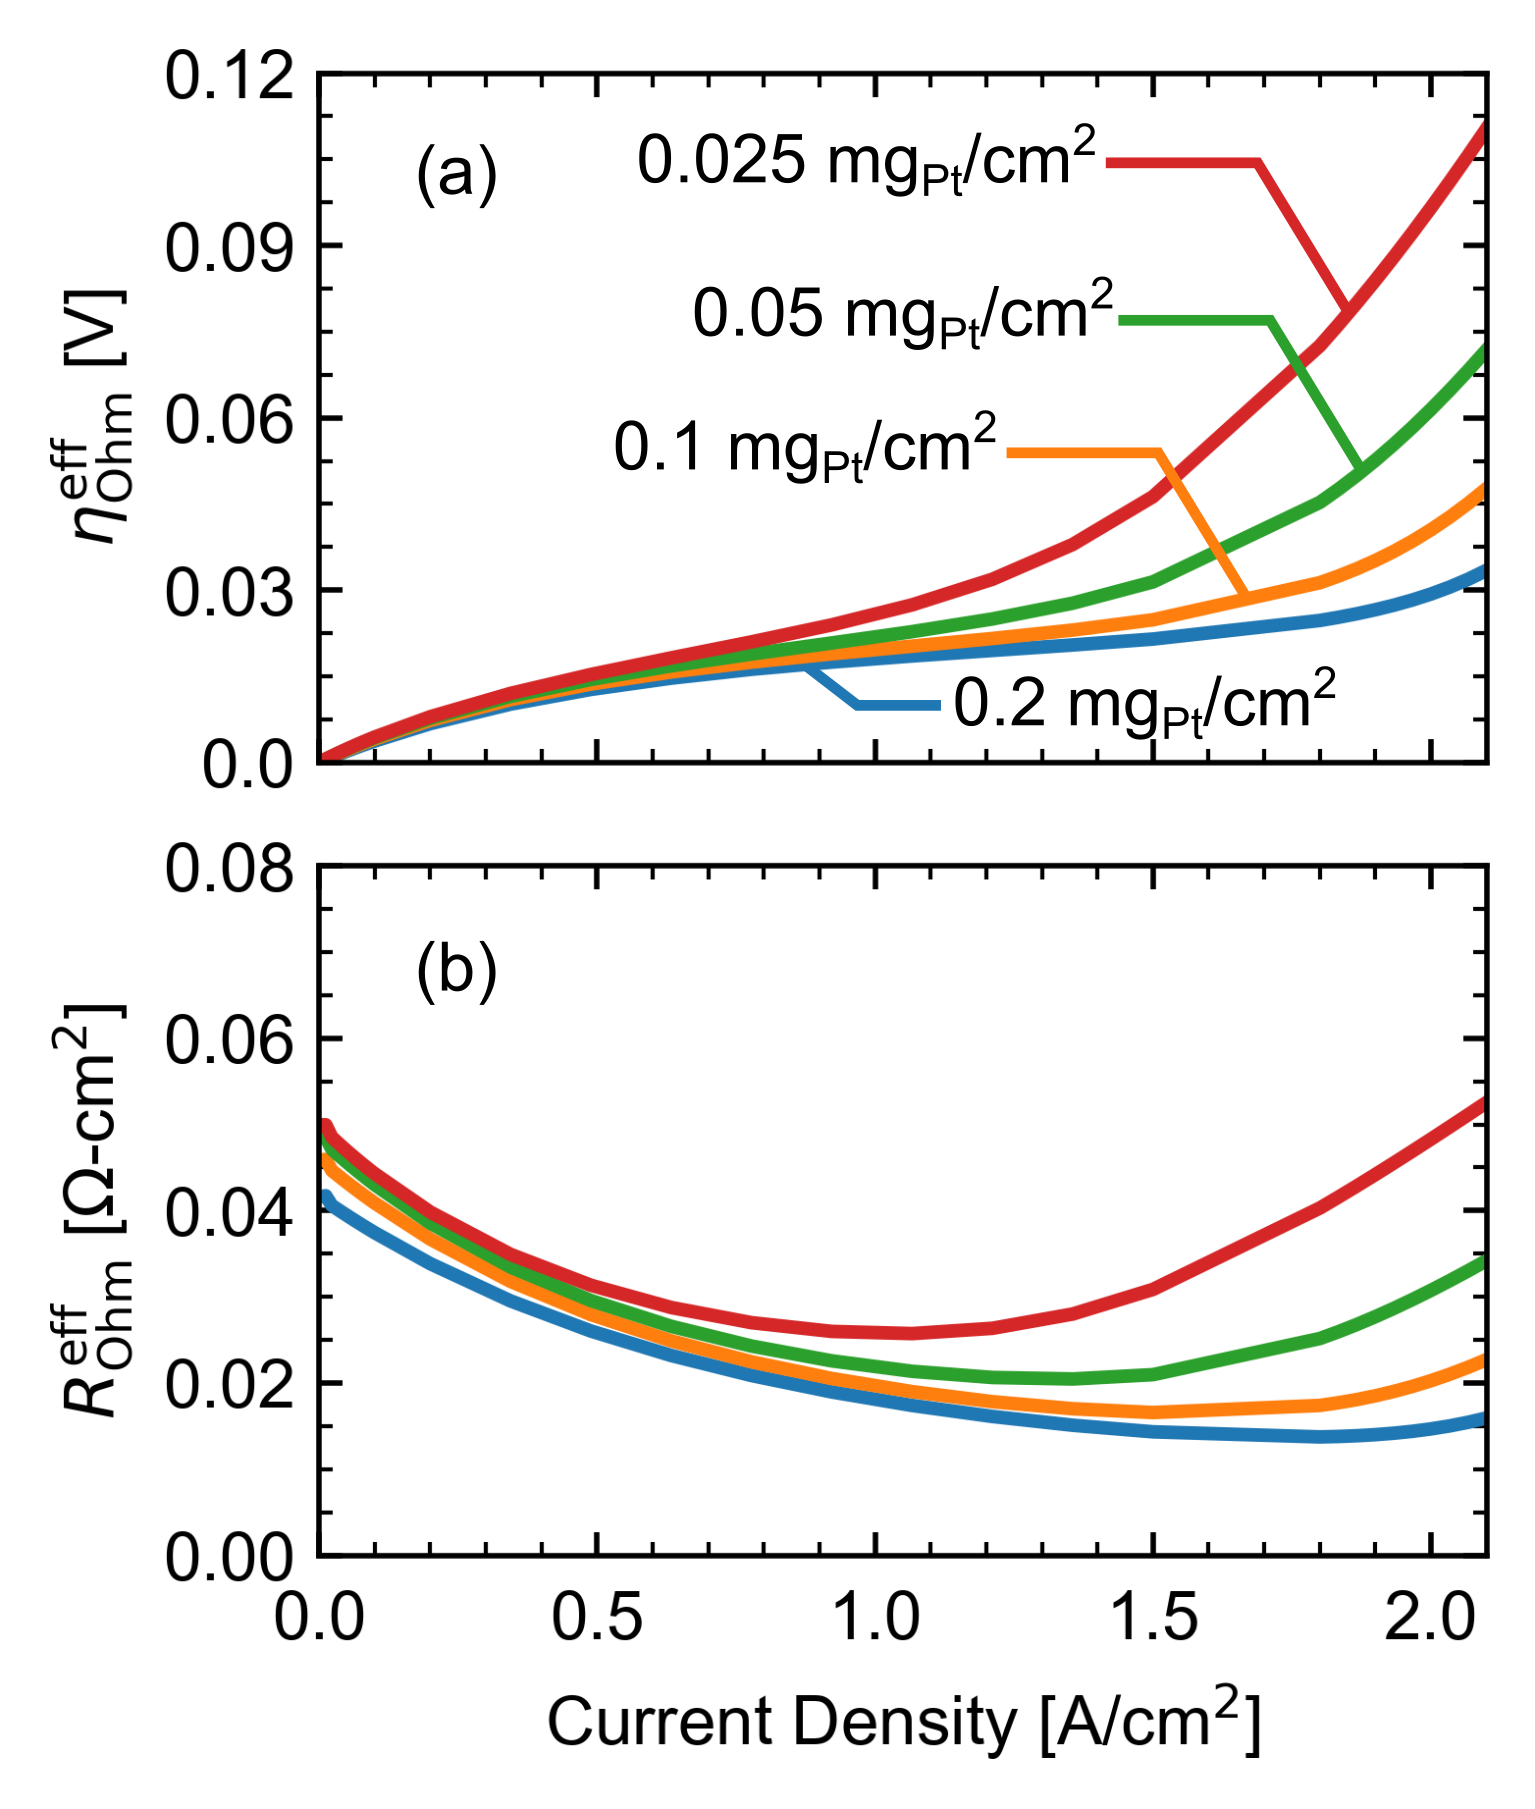
\includegraphics[width=3.07in]{figures/effective-ohmic-plots-3_07in.png}
    \caption{Effective Ohmic overpotential (a) and resistance (b) due to ion conduction in the CL for the `mixed' transport model. Results demonstrate that Ohmic losses and resistance change dynamically as a function of current density and Pt loading. These changes are due to changes in the Nafion conductivity with increasing water content ($R_{\rm Ohm}^{\rm eff}$ decreases with increasing current density, at low current densities), and to changes in the spatial distribution of Faradaic currents with increasing current density.}
    \label{fig:effective-Ohmic-measures}
\end{figure}

Results demonstrate directly that Ohmic losses play a critical role in explaining performance with varying Pt loading. In figure~\ref{fig:effective-Ohmic-measures}(a), Ohmic overpotentials are nearly identical at low currents, but change dramatically with increasing current. At ${\bf j}_{\rm ext} = 2.0$~A~cm$^{-2}$, the losses for 0.025~mg$_{\rm Pt}$~cm$^{-2}$ are more than three times greater than for the highest loading.  

Effective Ohmic resistances are plotted in figure~\ref{fig:effective-Ohmic-measures}(b) and show non-monotonic changes in $R_{\rm Ohm}^{\rm eff}$ over the range of current densities. At low current densities, $R_{\rm Ohm}^{\rm eff}$ decreases with increasing current density. Note that $R_{\rm Ohm}^{\rm eff}$ is a function of both \emph{material properties} (local variations in $\sigma_{\rm io}$) as well as \emph{process variables} (the extent to which protons are conducted deeper into the CL). Because the model is run with 99\% relative humidity in the gas flow channel, liquid water is not present at very low currents. As the current increases and the cell produces water, Nafion becomes more hydrated and its conductivity increases, causing an initial decrease in resistance. At low/moderate currents, the charge transfer resistance $R_{\rm ct}$ is less than $R_{\rm Ohm}$, and it is therefore favorable to produce the majority of the Faradaic current near the membrane interface. 

\begin{figure}[!tb]
    \centering
    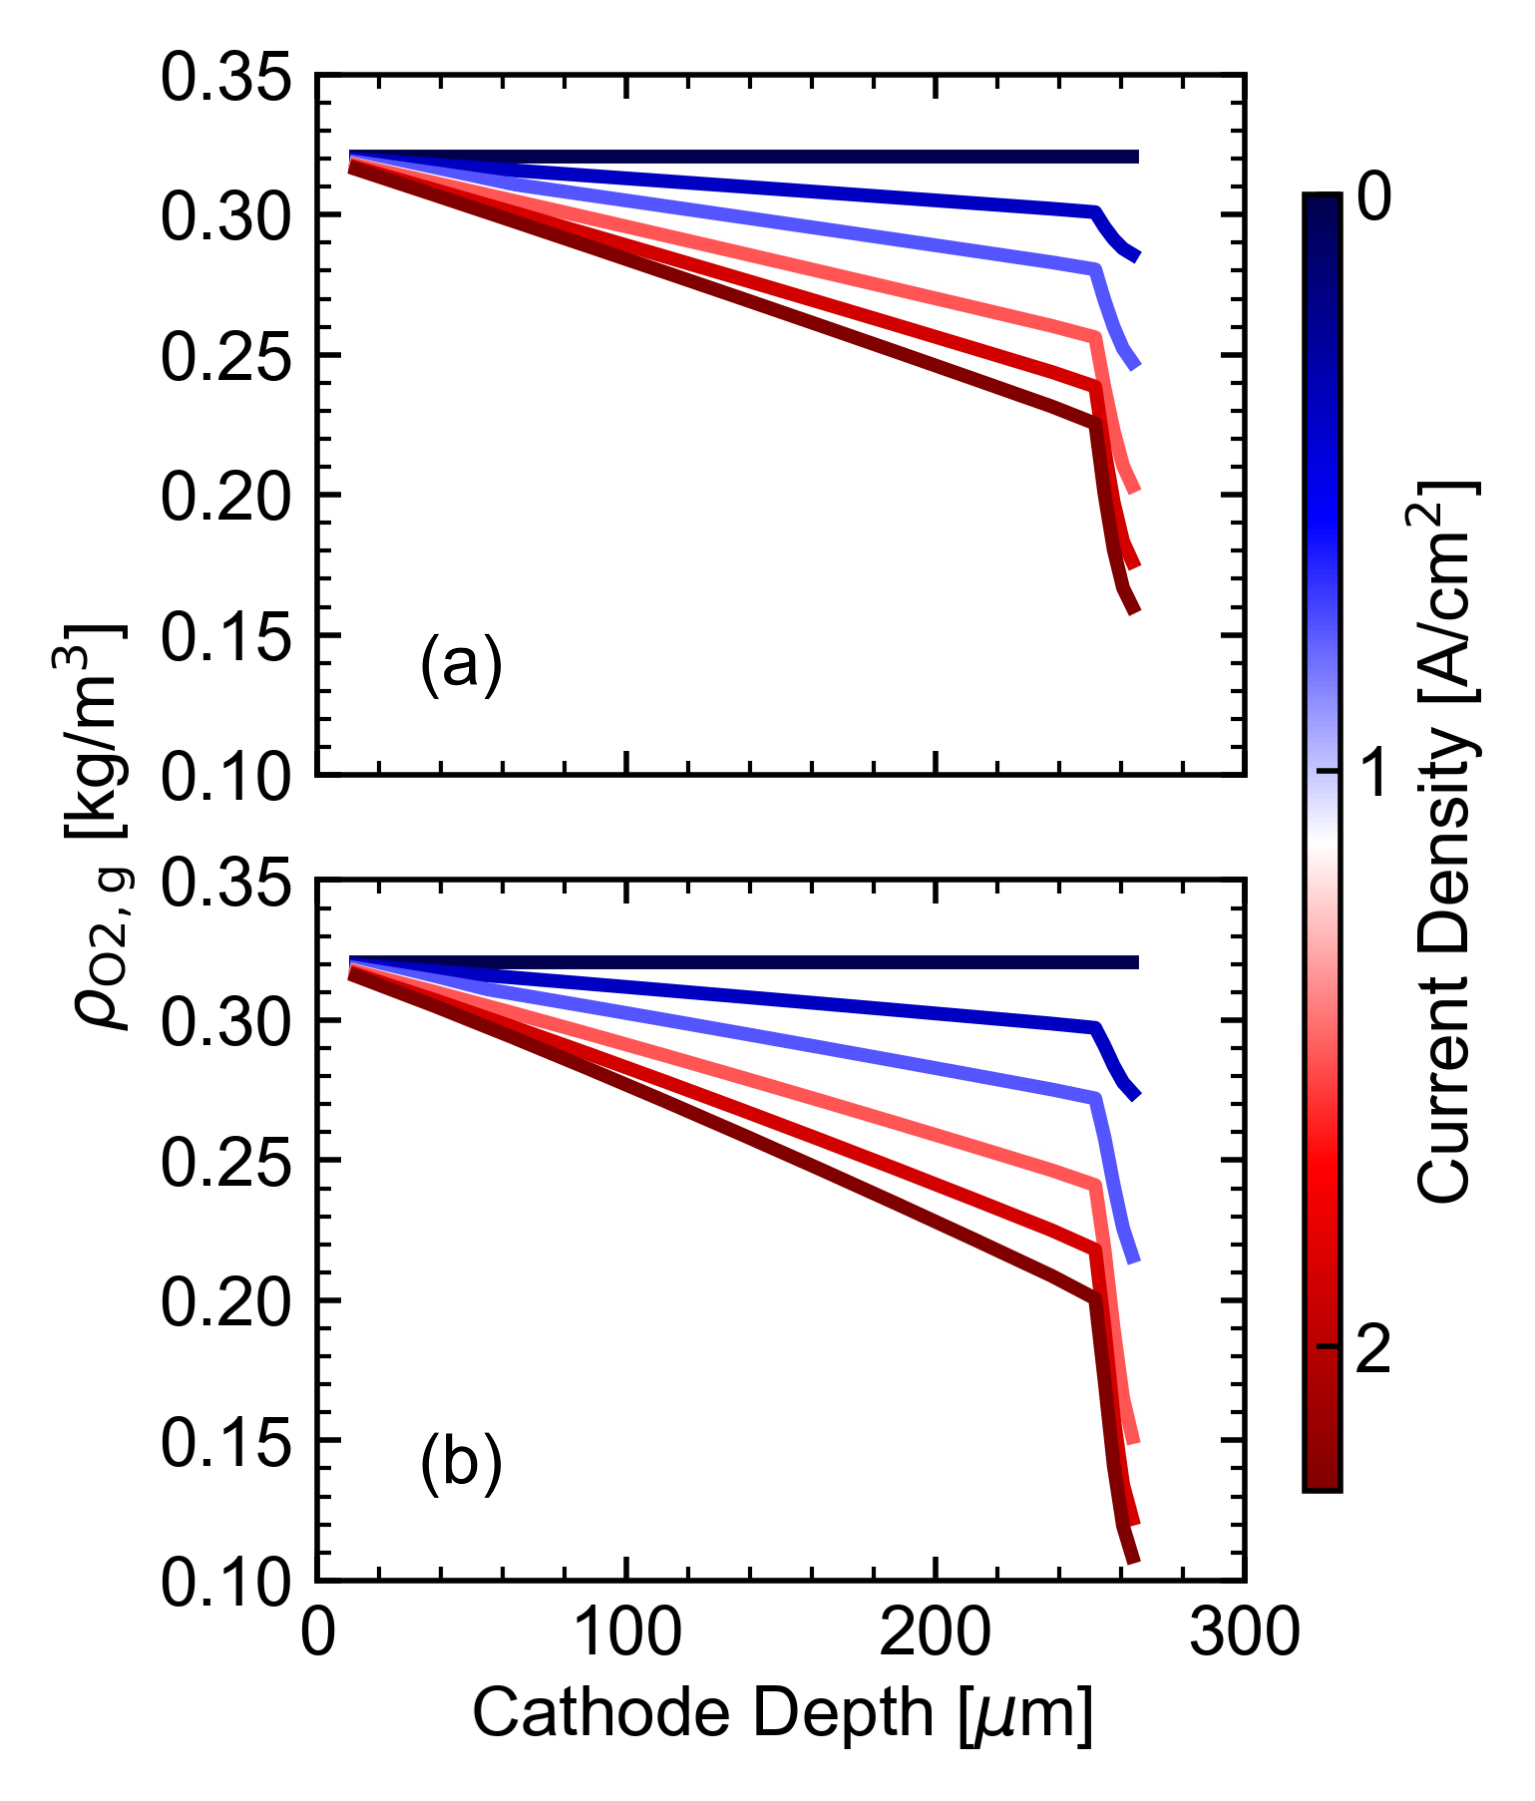
\includegraphics[width=3.07in]{figures/o2-grads-3_07in.png}
    \caption{Depth profiles for the gas-phase oxygen density ($\rho_{\rm O2, g}$) when the model is run (a) without liquid phase and (b) with liquid phase considerations. Plotted results are taken using the 'mixed' transport properties and the 0.025~mg$_{\rm Pt}$~cm$^{-2}$ Pt loading. The colorbar specifies the range of current densities for which the profiles are taken.}
    \label{fig:o2-grads-with-flooding}
\end{figure}

As current density increases, charge transfer overpotentials grow faster than Ohmic overpotentials, due to the exponential vs.~linear dependence on current, respectively. At some point, $R_{\rm ct}$ is larger than $R_{\rm Ohm}$, and the spatial Faradaic current density distribution becomes more uniform, thereby increasing the Ohmic losses. Kinetic limitations near the PEM are exacerbated by increased water saturation in the pores, which restricts gas-phase O$_2$ transport, as shown in figure~\ref{fig:o2-grads-with-flooding}, and also reduces the area available for O$_2$ absorption into the Nafion phase. Figure~\ref{fig:effective-Ohmic-measures}(b) shows that this transition -- from Faradaic current concentrated near the PEM to a uniform $j_{\rm Far}$ distribution -- occurs for all Pt loadings. Increasing Pt loading simply shits the current density of the transition (and associated increase in $R_{\rm Ohm}^{\rm eff}$). 

These results demonstrate the highly coupled nature of physiochemical processes in the PEMFC CL. While increasing voltage losses with low Pt loading are the \emph{direct} result of Ohmic processes, these Ohmic losses are driven by kinetic and gas-phase transport limitations. The distribution of currents will always adjust to minimize the total voltage loss. In this case, it means that increasing the resistive ionic currents is preferred, rather than increasing \emph{highly} resistive Faradaic currents near the membrane interface. Similar observations in solid oxide fuel cells  were made some time ago by one of the present authors~\cite{bib:decaluwe_2008}. In that study, lower anode porosity resulted in an increased ``utilization thickness,'' $\delta_{\rm util}$. Limitations were driven by transport processes (and increasing kinetic limitations with decreasing reactant availability), but as in the present study the observable result was higher predicted Ohmic losses.

% \subsubsection{Effects of flooding}
% \label{sect:effects-of-flooding}

% Although flooding is a well-known phenomena that occurs in PEMFCs, the effects that it has on each process that occurs in the CL is unclear. Therefore, the model was used to examine the contributions of flooding blocking Nafion-gas interfaces, decreasing diffusion pathways in the Nafion-phase, and increasing tortuosity of gas-phase transport. The results suggest that the most significant impact of flooding is on the diffusion in the gas phase. This is shown in figure~\ref{fig:o2-grads-with-flooding} where the liquid phase was turned off in (a) and turned back on in (b). When the liquid phase is present the added tortuosity decreases the effective diffusion coefficients in the gas phase, requiring larger gradients to move oxygen deeper into the CL. Lower amounts of gas-phase oxygen lead to less oxygen absorbing into the Nafion phase, slowing down the ORR kinetics. When kinetics are slow, it becomes even more essential to utilize all of the available Pt catalyst surface area to keep the cell operating at high currents. Consequently, cells with low loadings are more sensitive to flooding. 

\subsection{CL microstructure designs for high-performance, low-cost PEMFCs}
\label{sect:design_study}

In this section, we explore CL design parameters to improve PEMFC performance with low Pt loading, by mitigating Ohmic overpotentials and/or flooding impacts discussed in section~\ref{sect:cause-of-losses}. Design variations include simple changes such as CL thickness and average ionomer loadings, as well as more advanced designs such as functionally graded ionomer and Pt loadings throughout the CL depth, as illustrated in figure~\ref{fig:design-study}. CL property variations are summarized in table~\ref{tab:design-study}. All simulations are run with the lowest Pt loading, 0.025~mg$_{\rm Pt}$~cm$^{-2}$.

\subsubsection{CL thickness and Nafion shell thickness}

The CL thickness was independently varied, as indicated in table~\ref{tab:design-study}. Thinner CLs provide higher Pt densities (per unit volume) and shorter transport distances for protons entering the CL and liquid water exiting the CL, reducing Ohmic losses and CL saturation (which in turn reduces gas-phase transport resistance). The CL thickness was reduced from 15~$\mu$m (figure~\ref{fig:validation_air}) to 12 and 9~$\mu$m in the parametric study. Full polarization and power curves are provided in figure~\ref{fig:CL-thickness-study}. As expected, a thinner CL improves the cell performance, via higher power densities and higher limiting currents. The maximum power densities, however, occur near the limiting current, a less than ideal operating condition. 

Thicker ionomer films in the CL will improve PEMFC performance because they absorb more water and have higher conductivities~\cite{bib:decaluwe_2018, bib:kusoglu_2017, bib:eastman_2013}. More absorbed water also leads to more dissolved oxygen in the films. Additionally, thicker shells result in higher Nafion volume fractions and lower tortuosities, reducing the proton transport resistance. On the other hand, thinner Nafion shells provide shorter diffusion paths between the pore and Pt catalyst. The Nafion shell thickness was varied from 7 to 18~nm (it was a constant 12~nm for figures~\ref{fig:validation_air} and \ref{fig:o2-grads-with-flooding}). Results, in figure~\ref{fig:bar-charts} and figure~\ref{fig:naf-thickness-study} in the SI, predict that maximum power densities increase with increasing $t_{\rm N}$. The limiting current is approximately the same for all cases, demonstrating that increased dissolved oxygen in the Nafion compensates for the larger diffusion lengths. Although not shown, the limiting current would decrease with sufficiently thick films, as demonstrated in our earlier publication~\cite{bib:randall_2020}. % This former study over-approximated oxygen transport resistance, but the same trend would be observed here, only for much thicker films. %Also notable is the performance of the 7~nm case in figure~\ref{fig:naf-thickness-study}, which has much higher overpotentials than the other cases, demonstrates how simple changes can have compounding positive or negative effects. 

\begin{figure}[!tb]
    \centering
    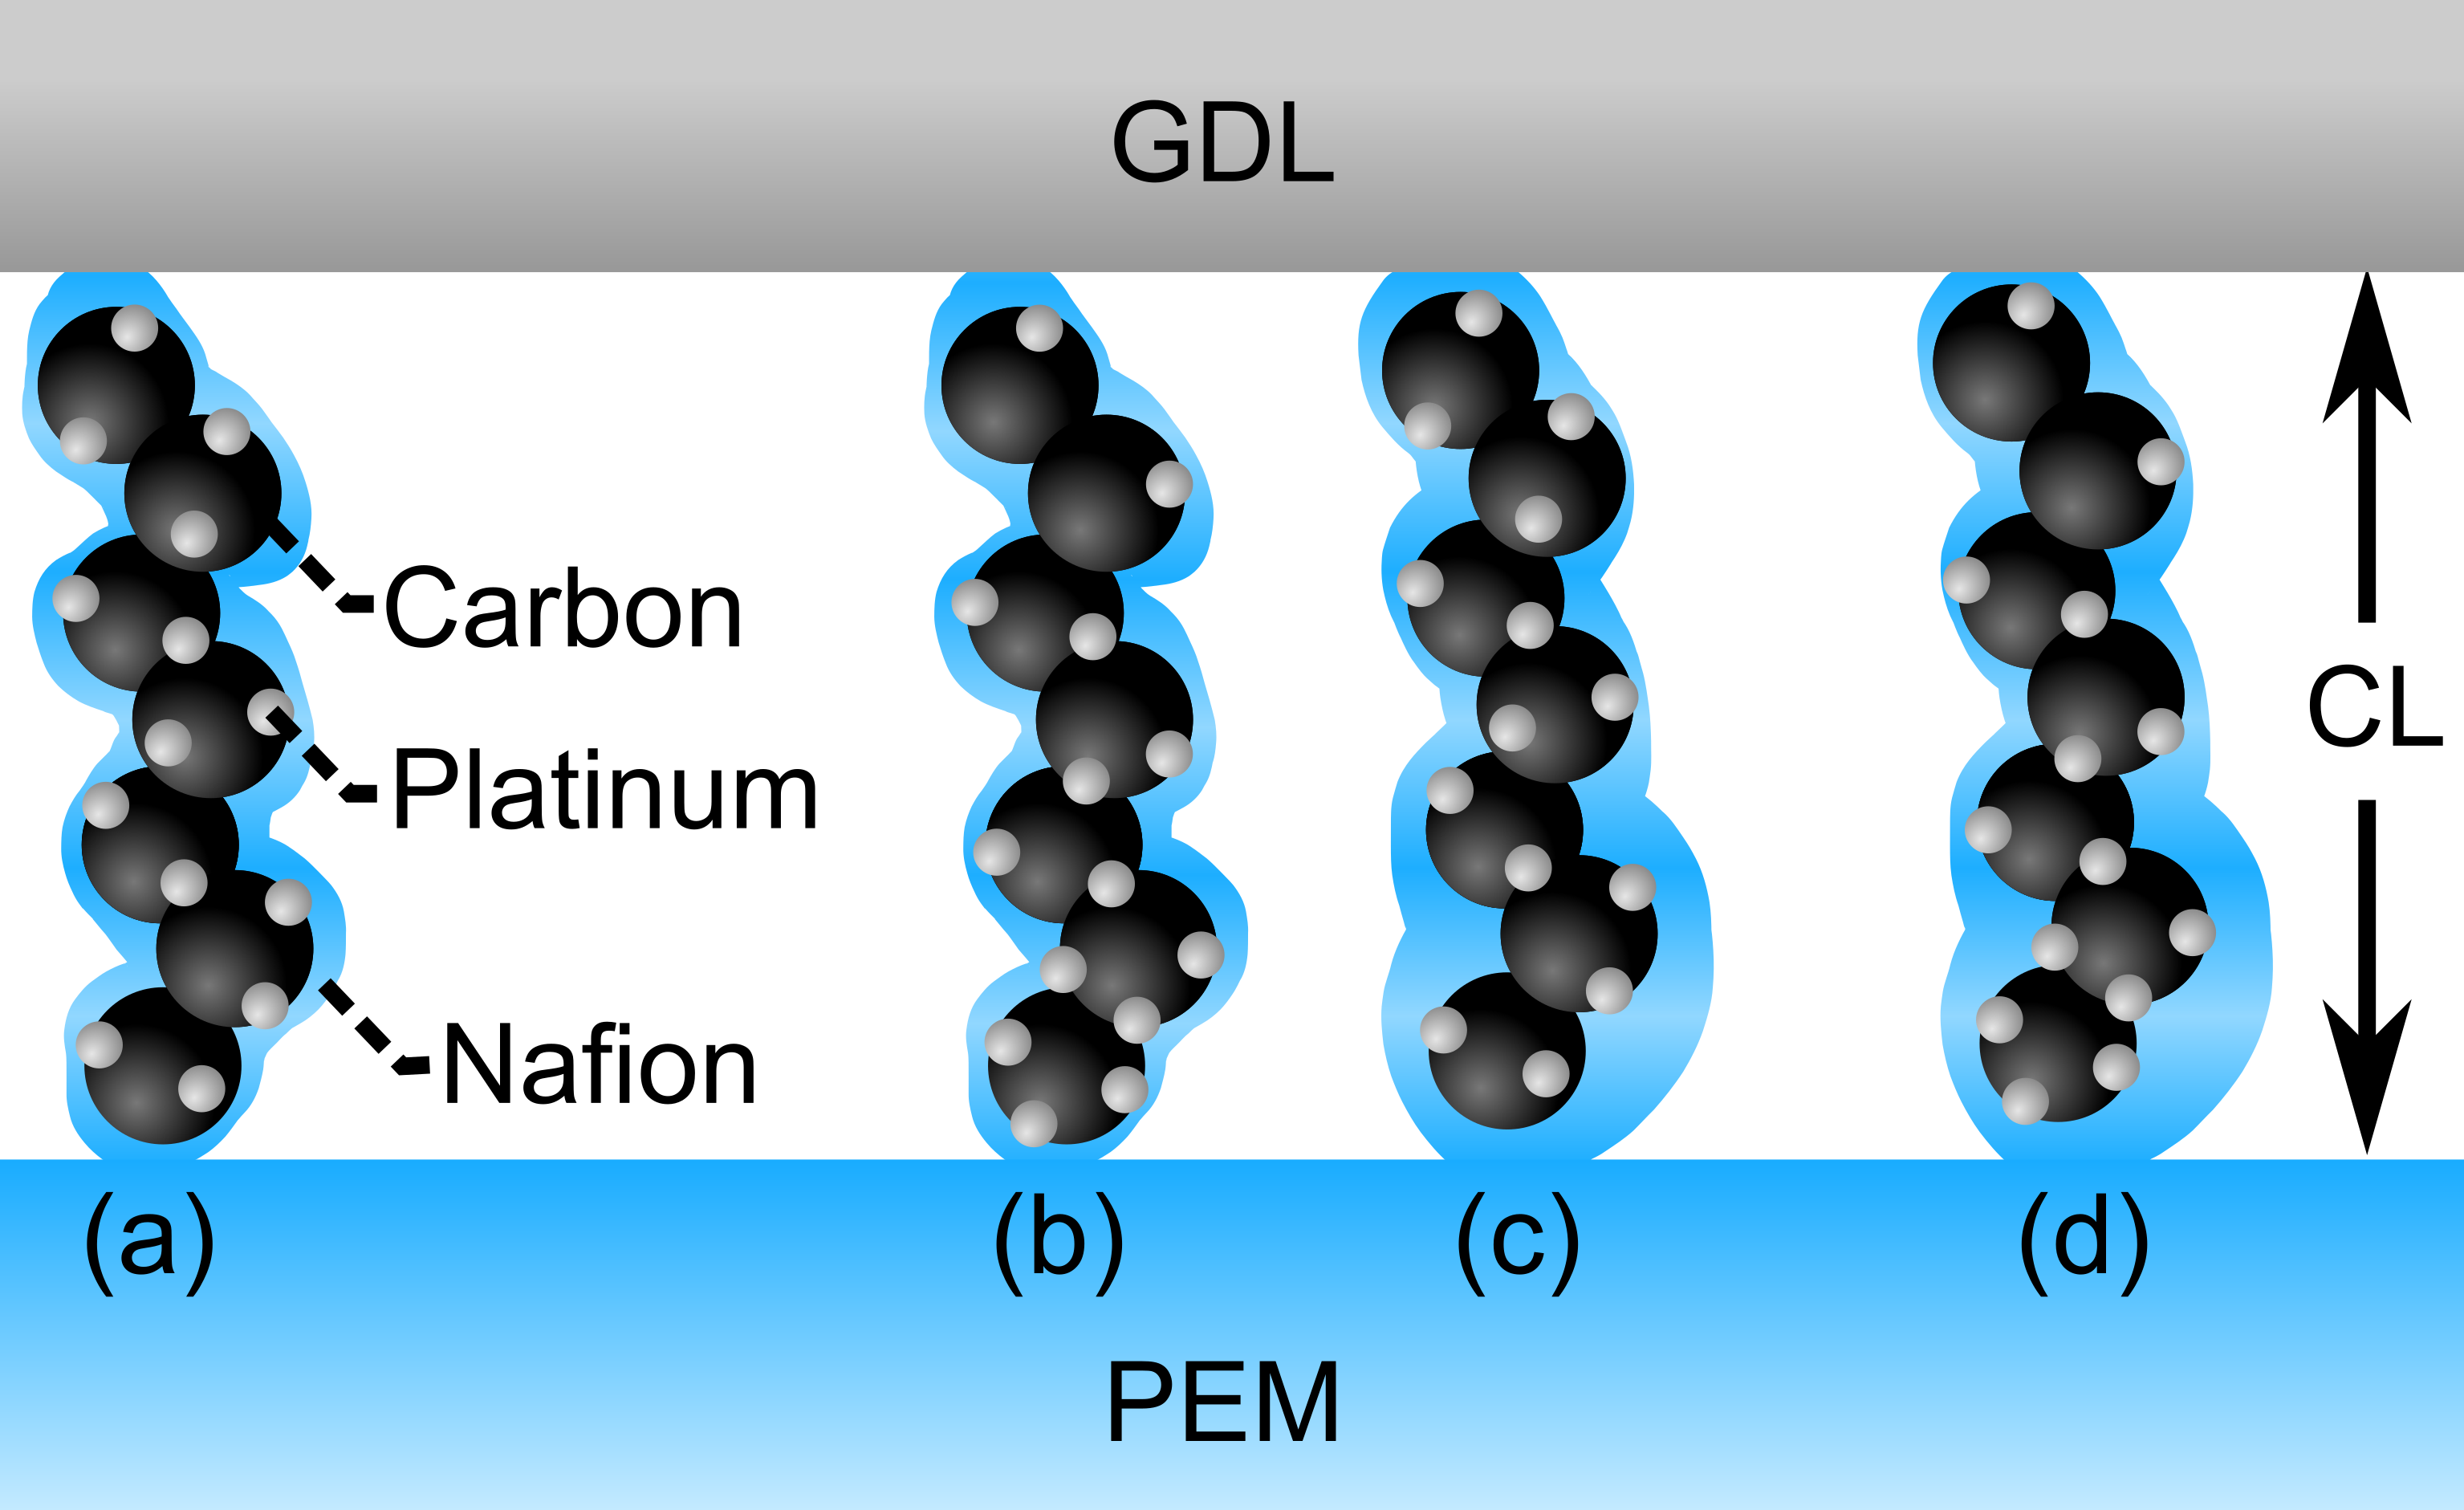
\includegraphics[width=3.07in]{figures/design-study-3_07in.png}
    \caption{Illustration of CL microstructures with (a) uniform Pt and ionomer loading, (b) graded Pt loading, (c) graded ionomer loading, and (d) dual graded Pt and ionomer loading.}
    \label{fig:design-study}
\end{figure}

\subsubsection{Ionomer and Pt loading distributions}

In this section, detailed structure-property relationships, updated during the simulation as a function of time and location, enable accurate simulation of non-uniform Nafion and Pt loadings. The above results assume uniform Nafion and Pt loading throughout the CL. In actual PEMFCs, the Nafion thickness is heterogeneous and ranges between roughly 5 and 15~nm. Similarly, Pt is not uniformly dispersed, and can form aggregates and clusters within CL regions. With increasing control over CL fabrication, functionally graded CLs may provide a pathway to improve PEMFC performance while limiting cost. Five studies were used to explore the impact of non-uniform phase distributions:
\begin{enumerate}
    \item `Random Naf': Random ionomer shell thickness as a function of CL depth (alternating shells of thickness 7 and 12~nm throughout the CL).
    \item `Linear Naf': Graded ionomer thickness (5~nm at the GDL interface, increasing linearly to 12~nm at the PEM interface).
    \item `Linear Pt': Graded Pt density (5.7~mg~cm$^{-3}_{\rm tot}$ at the GDL interface, linearly increases to 27.7~mg~cm$^{-3}_{\rm tot}$ at the PEM interface).
    \item `Exponential Pt': Graded Pt density (2.8~mg~cm$^{-3}_{\rm tot}$ at the GDL interface, increasing exponentially to 43.3~mg~cm$^{-3}_{\rm tot}$ at the PEM interface).
    \item `Dual graded': Combination of the `Linear Naf' and `Exponential Pt' cases.
\end{enumerate}

\begin{table*}[!htb]
    \small
    \centering
    \caption{Parametric study summary}
    \vspace*{1mm}

    \begin{tabular}{l c c c}
    \hline \hline
    & CL thickness [$\mu$m] & Nafion thickness [nm] (distribution)  & Pt distribution$^{*}$ \\
    \hline 
    Base case           & 15    & 12 (uniform)                      & uniform \\
    CL thickness        & 9,12  & 12 (uniform)                      & uniform \\
    Nafion thickness    & 15    & 7,18 (uniform)                    & uniform \\
    Nafion distribution & 15    & 7,12 (alternating, i.e. random)   & uniform \\ 
                        & 15    & 5--12 (linearly increasing)       & uniform \\ 
    Pt distribution  & 15    & 12 (uniform)                         & linear$^{\dagger}$ \\ 
                     & 15    & 12 (uniform)                         & exponential$^{\ddagger}$ \\ 
    \hline \hline \vspace*{-3mm} \\
    \multicolumn{4}{l}{$^{*}$ For each study, all loadings are 0.025~mg$_{\rm Pt}$~cm$^{-2}$. This is verified by integrating the Pt over each CL thickness.} \\
    \multicolumn{4}{l}{$^{\dagger}$ Pt density ranges from 5.7 (near GDL) to 27.7~mg~cm$^{-3}_{\rm tot}$ (near PEM).} \\
    \multicolumn{4}{l}{$^{\ddagger}$ Pt density ranges from 2.8 (near GDL) to 43.3~mg~cm$^{-3}_{\rm tot}$ (near PEM).}
    \end{tabular}
    \label{tab:design-study}
\end{table*}

\begin{figure*}[!htb]
    \centering
    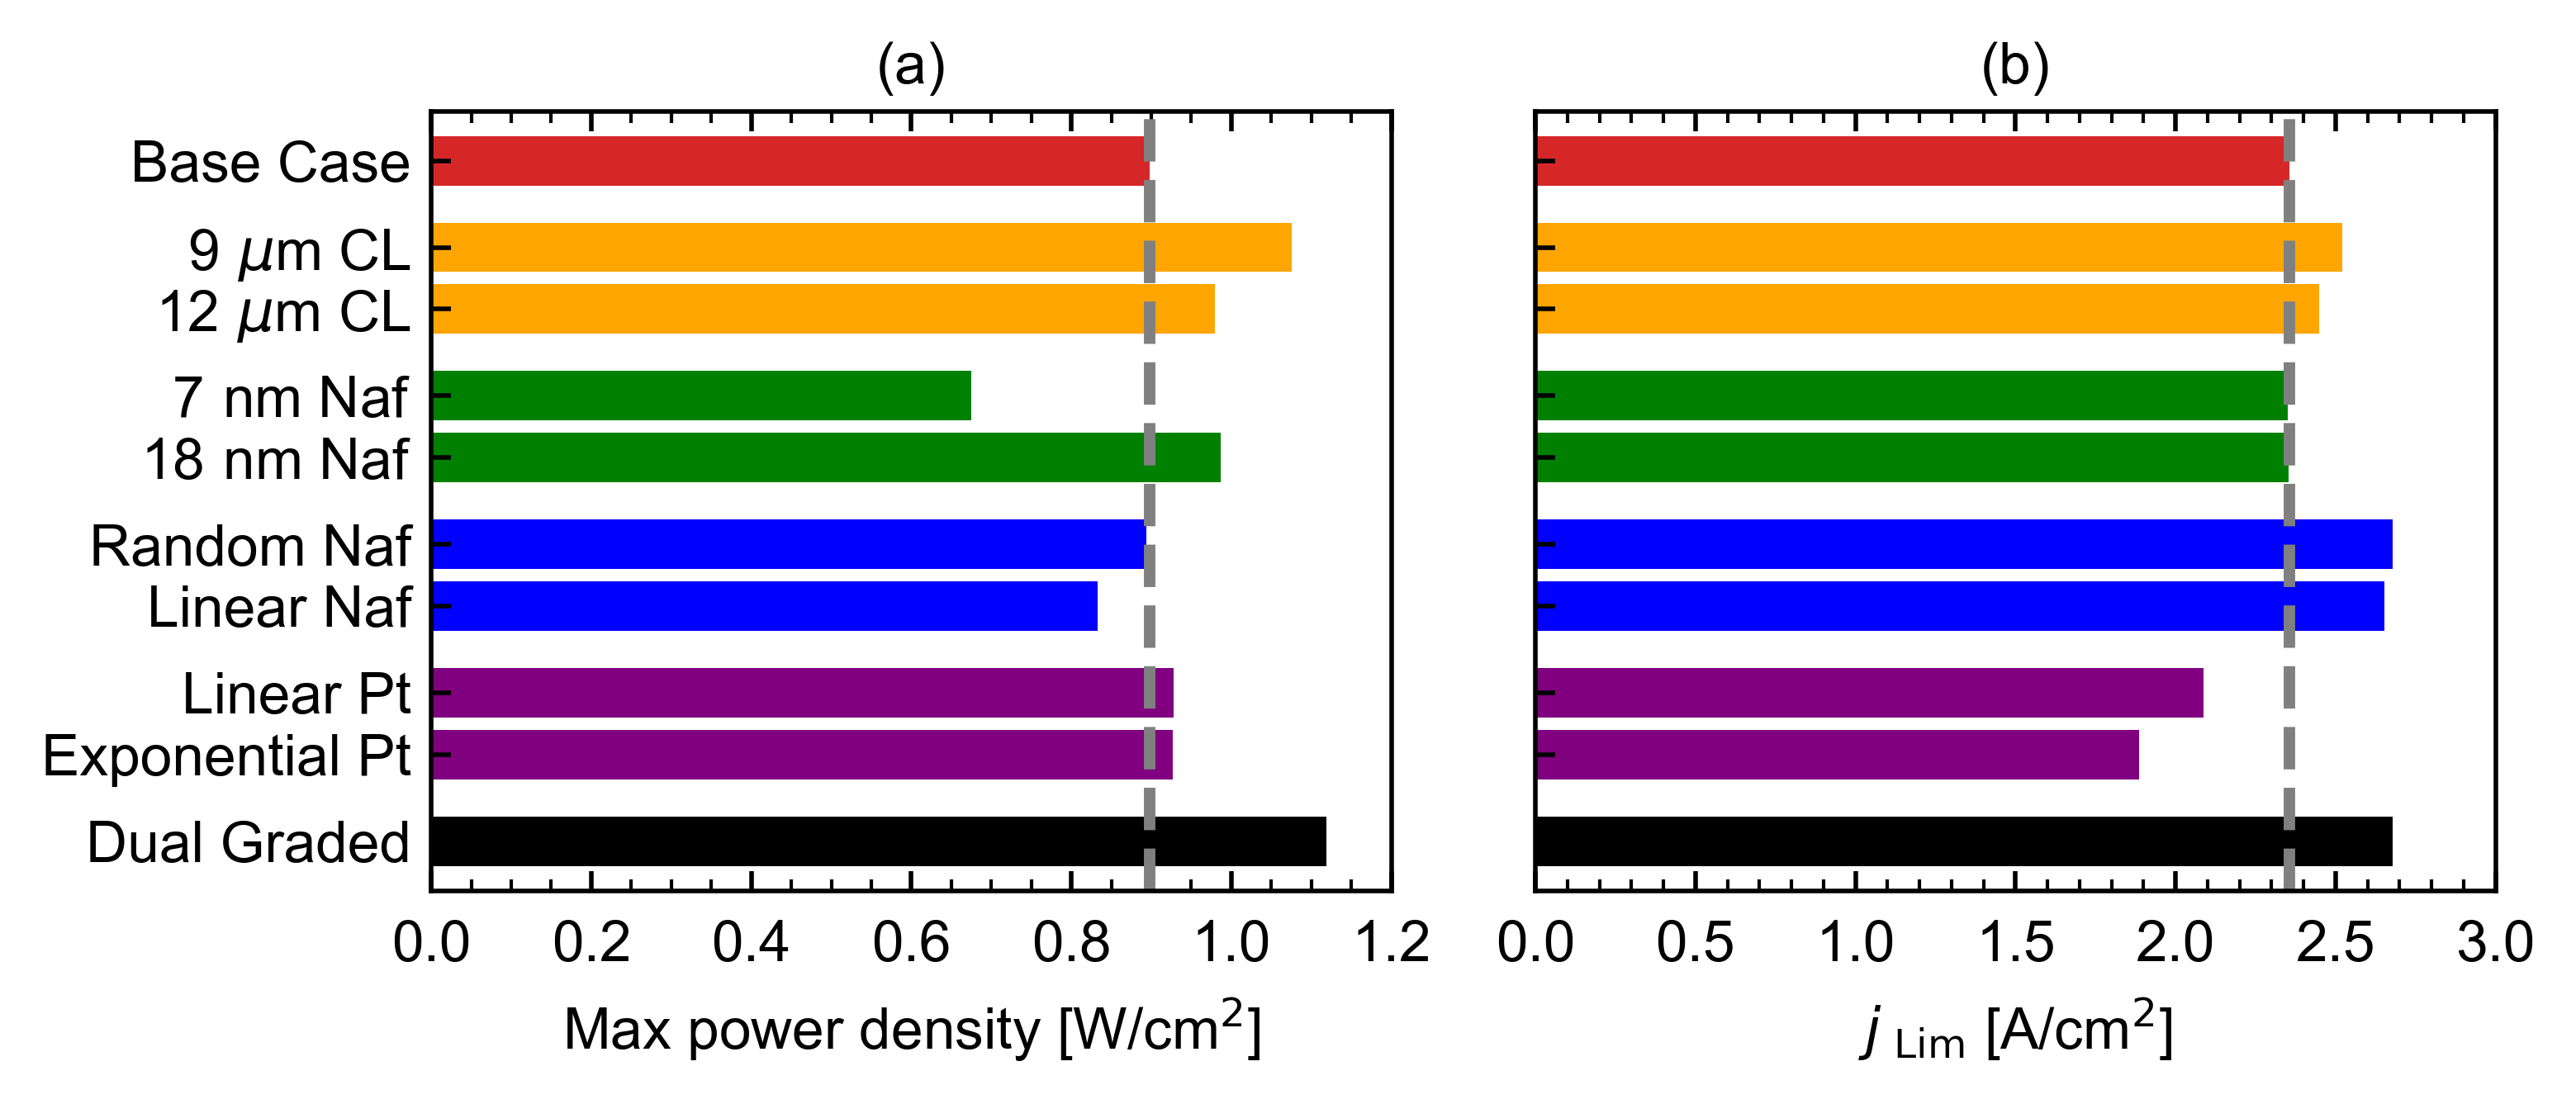
\includegraphics[width=6.238in]{figures/bar-charts-6_238in.png}
    \caption{Parametric study results highlighting the (a) maximum power density and (b) limiting current $j_{\rm Lim}$ of each simulation. The red bar is for the base case. The remaining colors emphasize each parameter category: CL thickness (orange), Nafion shell thickness (green), Nafion distribution (blue), Pt distribution (purple), and dual graded Pt and Nafion distributions (black). Dashed lines mark the the base case performance for easier comparison against the others. Full parameter details for each simulation are summarized in table~\ref{tab:design-study}.}
    \label{fig:bar-charts}
\end{figure*}

%Here, we approximate this heterogeneity by allowing the Nafion shell thickness to vary with CL depth, with alternating shells of 7 and 12~nm throughout the CL. Where the Nafion shells are made thinner, the porosity increases. This distribution is labeled ``Random'' in figure~\ref{fig:bar-charts}, with the full polarization and power curves given in figure~\ref{fig:naf-distribution-study}. Through a current density of 2.2~A~cm$^{-2}$, the results of the base case and random distribution align quite well. The random case does show a slightly lower voltage at low currents, caused by the increased tortuosity and reduced water uptake from the sections of thinner ionomer shells. At higher currents however ($>$2.2~A~cm$^{-2}$), the random case results in a higher limiting current. This is a result of higher local porosities where the ionomer thickness is decreased. Since the validation data was only available for current densities of 2.0~A~cm$^{-2}$ or less, it can be argued that the random distribution is fairly equivalent to the base case. 

Table~\ref{tab:design-study} summarizes parameters for each case. All graded cases have lower loadings near the GDL and higher loadings near the PEM. Grading in the reverse direction would degrade PEMFC performance by increasing Ohmic resistance and flooding. This is confirmed in part by experiments with dispersed Pt from Owejan et al.~\cite{bib:owejan_2013}. Their study concluded that PEMFCs with dispersed Pt had lower performance than those with uniformly distributed Pt. The total Pt loading for all studies was 0.025 mg$_{\rm Pt}$ cm$^{-2}$, as indicated in table~\ref{tab:design-study}.  

Full polarization and power density curves from each simulation are available in the SI. In short, varying Pt or Nafion independently is not predicted to significantly improve PEMFC performance. Varying the Pt loading actually reduces the limiting current, due to flooding and gas-phase transport limitations. For non-uniform Nafion loadings, the limiting current increases, by lowering transport resistances for all relevant species (ions, gas-phase O$_2$, and liquid water), but these improvements do not improve the maximum power density.
%A graded ionomer distribution was also considered. In this case, low loadings were concentrated near the GDL and high loadings were placed near the membrane. This resulted in thinner average shells near the GDL with higher porosities and thicker shells near the membrane with lower porosities. In figure~\ref{fig:bar-charts}, we refer to this case as `Increasing.' The outcomes of this change suggest a lower maximum power density and a higher limiting current compared to the base case. As discussed with the random distribution, the thinner shells result in higher Ohmic overpotentials, regardless of where they are located in the CL. Although the power output is decreased, the limiting current is increased by reducing gas-phase flooding effects with the higher porosities. 
%All in all, neither of these design considerations was shown to have a dramatic impact on performance compared to the base case. %Note that a decreasing distribution, with high loadings near the GDL and low loadings near the membrane, did not make sense in the context of the aforementioned performance concerns. This type of distribution would increase both Ohmic overpotentials and flooding.

% One last change that was considered involves the Pt loading distribution. Rather than distributing the Pt content equally throughout the CL, as in the base case, it was also graded. The grading was done so that higher amounts of Pt were concentrated near the membrane interface in an attempt to reduce Ohmic overpotentials. Both a linear and an exponential functional distribution were tested, ensuring that the total amount of Pt remained constant. As shown in figure~\ref{fig:bar-charts}, this resulted in a marginal increase to power density with a dramatic decrease in limiting current compared to the base case. Higher amounts of concentrated flooding near the CL-membrane interface were responsible for the moderate change in power density. By blocking areas where high amounts of Pt surface area is available and increasing gas-phase transport resistance locally in these areas, the cell cannot sustain high currents. Consequently, much higher theoretical power densities are not plausible with solely graded Pt distributions. Note that other distributions of Pt were not considered here because they would not have been in line with reducing Ohmic losses and flooding. In fact, Owejan et al.~\cite{bib:owejan_2013} performed additional experiments with dispersed Pt. In these experiments, they diluted CL in solutions by having some carbon supports not covered in Pt. The results showed worse performance compared to equally distributed Pt catalysts. Consequently, any efforts to move Pt away from the membrane interface, either through a random distribution or a ``decreasing'' (from the GDL to the PEM) distribution would likely be ineffective.

As summarized in figure~\ref{fig:bar-charts}, none of the CL variations presented thus far significantly improves performance. Thinner CLs and thicker ionomer shells are predicted to increase the maximum power density, but these maxima occur very near the cell's limiting current. Varying the Nafion loading distribution improves the limiting current but not the power density, and varying the Pt distribution has a minor positive impact on maximum power and reduces the limiting current. Figure~\ref{fig:bar-charts} demonstrates that optimal designs must simultaneously reduce Ohmic losses \emph{and} limit pore flooding.

From these design trends, we hypothesize that a dual graded CL, where both Pt and Nafion vary as a function of depth, will significantly improve PEMFC performance. Such a design combines the benefits of graded Pt and Nafion. Graded Pt decreases the Ohmic resistance, while graded Nafion increases porosity to mitigate flooding effects. As shown in figure~\ref{fig:bar-charts}, results support this hypothesis. The `dual graded' model predicts the highest power density \emph{and} the highest limiting current, of all the designs considered.

\begin{figure}[!tb]
    \centering
    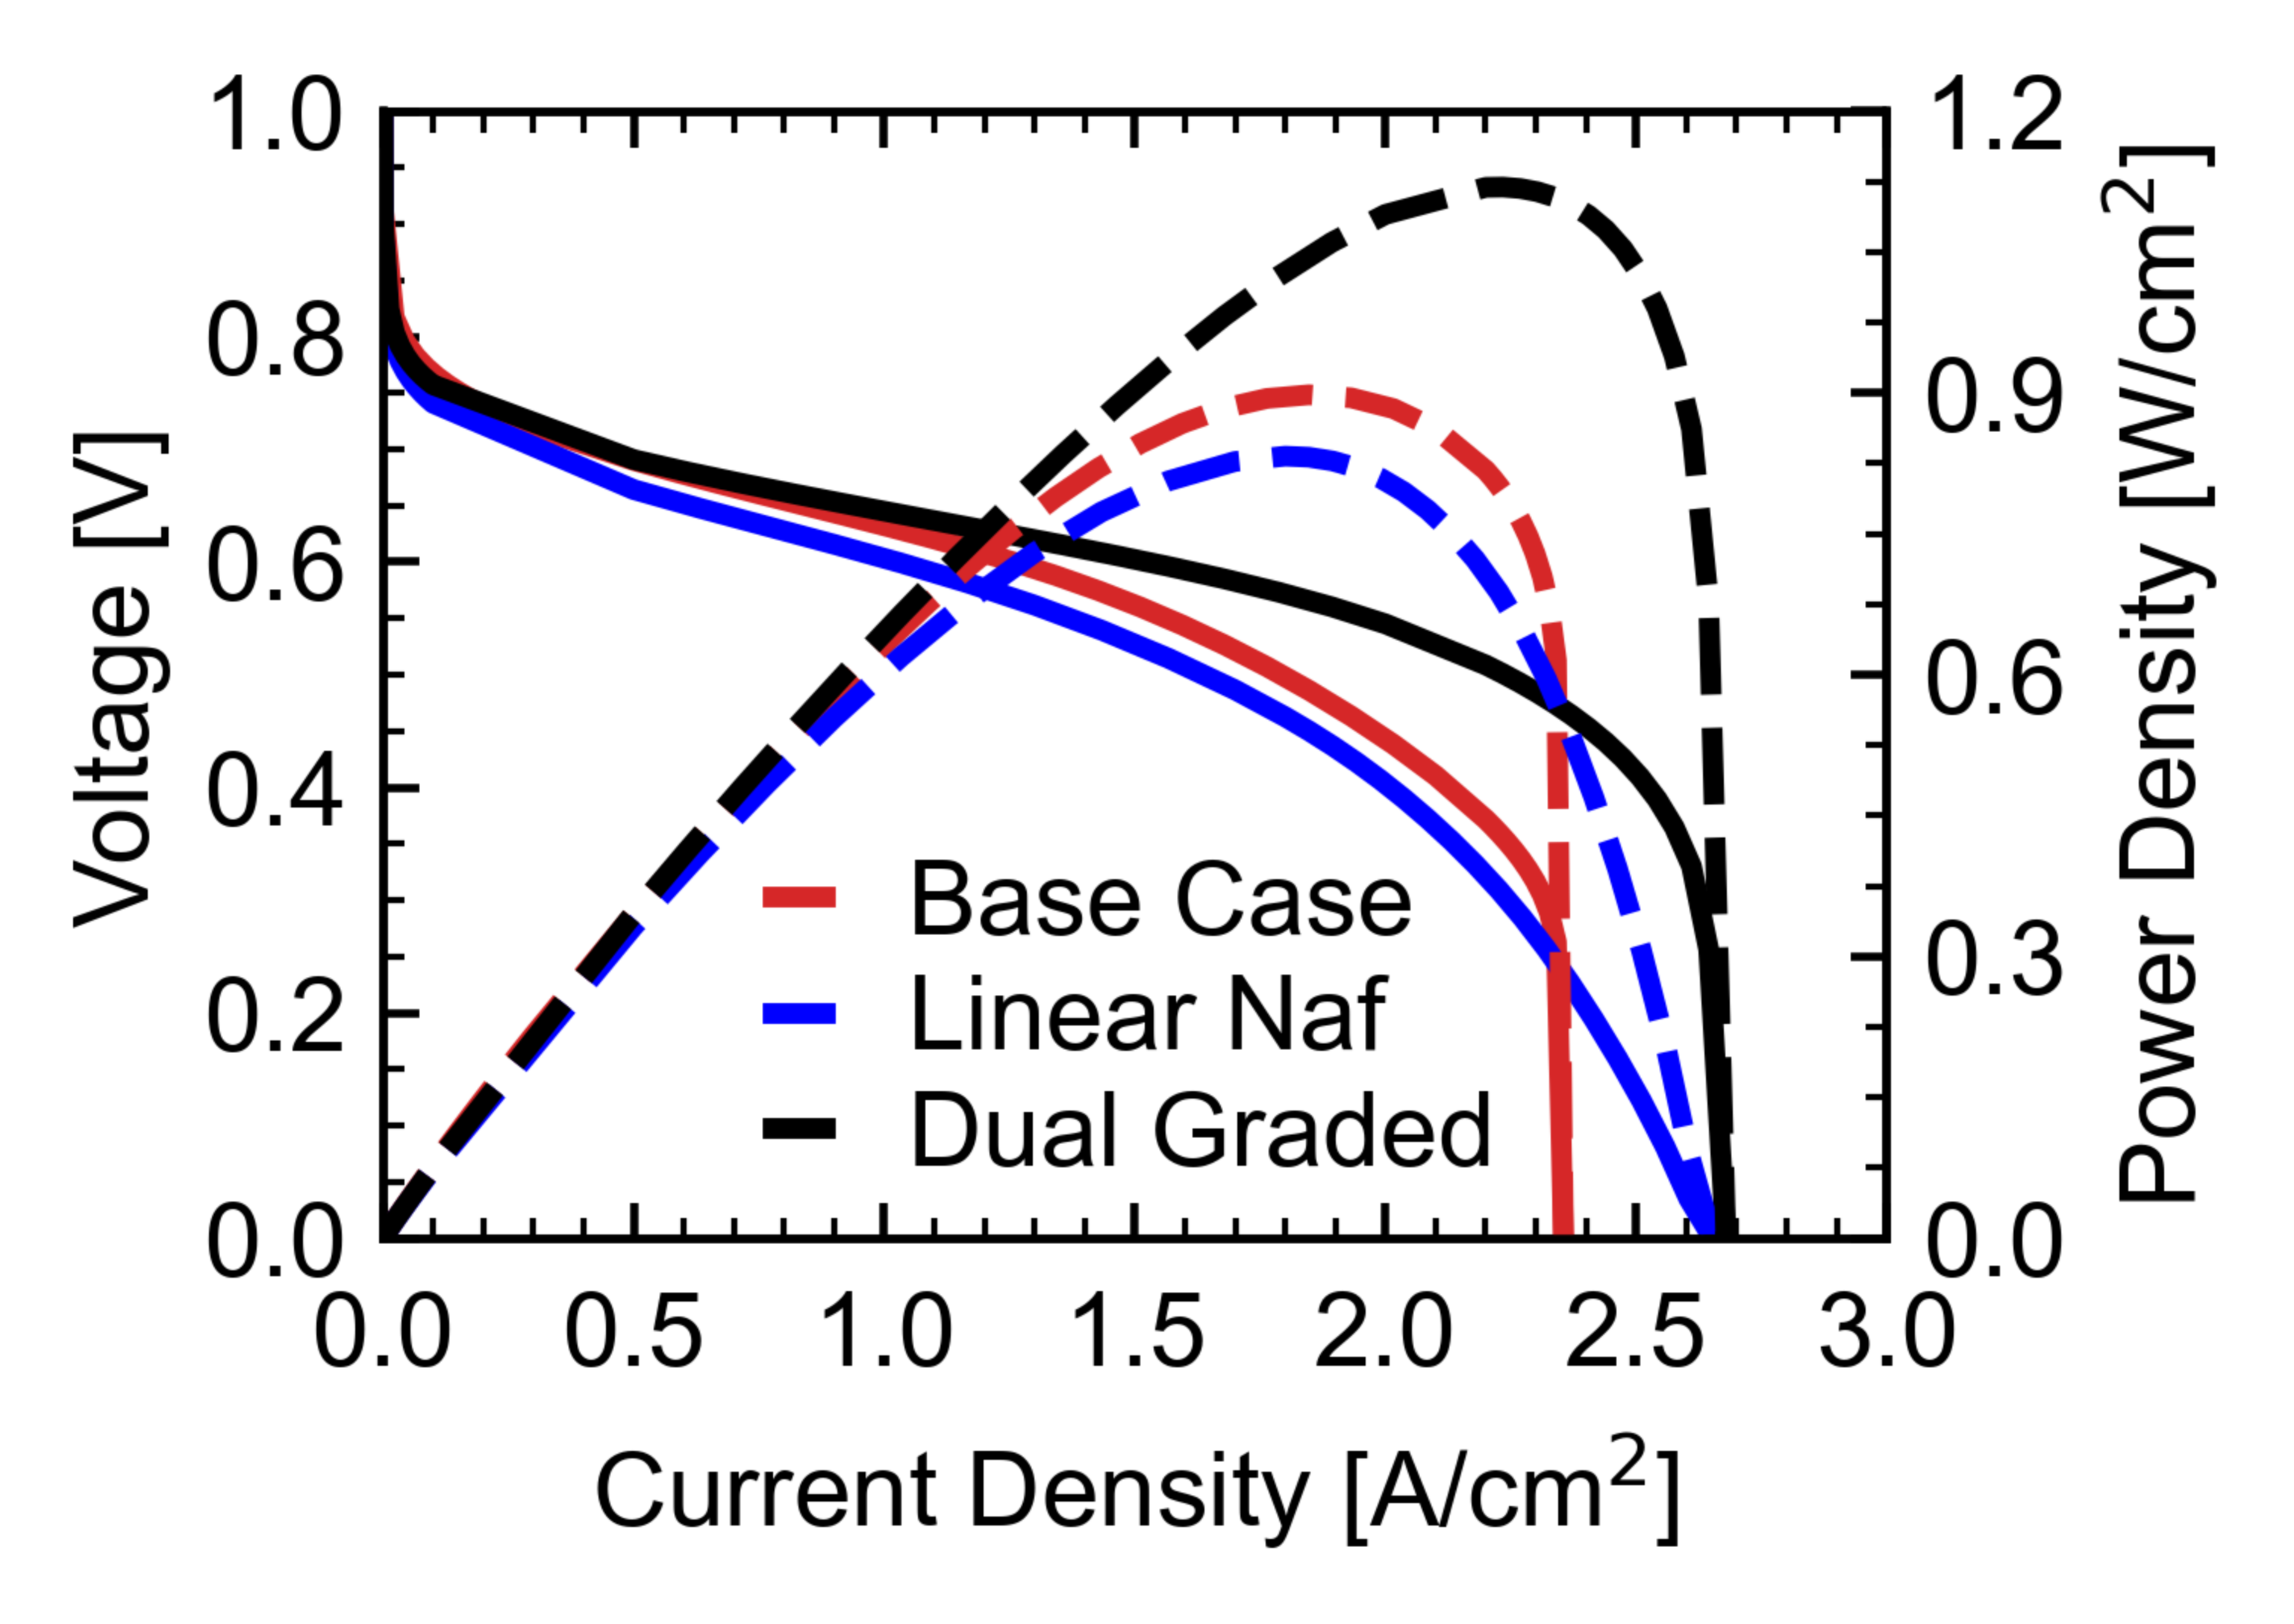
\includegraphics[width=3.07in]{figures/dual-grad-3_07.png}
    \caption{Polarization (solid) and power density (dashed) curves for the base case, linearly graded Nafion, and dual graded CL microstrucutes. Although individually grading the Nafion ionomer loading results in a higher limiting current, the cell performance decreases. Grading both the Pt and ionomer loadings maintains this higher limiting current while reducing Ohmic overpotentials.}
    \label{fig:dual-graded}
\end{figure}

Figure~\ref{fig:dual-graded} compares the base case from figure~\ref{fig:validation_air}, linearly graded Nafion, and dual graded designs. The graded Nafion and dual graded designs predict roughly the same limiting current densities, suggesting that the limiting current is exclusively controlled by flooding. Changes to power density are more complicated. The maximum power density of the dual graded case is much higher than that of the individually graded Pt cases. This is due to the cell voltage being influenced by multiple processes (e.g. oxygen/water diffusion in Nafion, flooding, proton transport, and charge transfer resistance). As demonstrated, designs must address multiple limiting phenomena in concert, to improve performance. In this case, the dual graded catalyst layer predicts a nearly 25\% increase in the maximum power density, and can help guide advanced PEMFC CL designs.


%%%%%%%%%%%%%%%%%%%%%%%%%%%%%%%%%%%%%%%%%%%%%%%%%%%%%%%%%%%%%%%%%%%%%%%%%%
\section{Conclusion}

To improve performance in low-cost PEMFCs, limiting phenomena at low Pt loadings must be identified and mitigated. Because of the catalyst layer's complex, heterogeneous micro- and nano-structure, \emph{operando} measurements for mechanistic understanding of physical processes in a PEMFC are challenging. We present here a model to predict the impacts of oxygen/proton transport and flooding in PEMFC CLs. Compared to other models, we emphasize accurate models for transport through the nano-thin Nafion films in the CL. This is achieved by combining quantified thin-film structures from neutron reflectometry experiments with separate conductivity measurements. This allows for accurate transport properties, resolved spatially and temporally, that evolve according to the local Nafion water content and film thickness. By validating the model against experimental data, we demonstrate that these structure-property relationships improve the model's capability to capture PEMFC behavior at low Pt loadings. Accurate fits ($\chi^2 < 2$) are obtained across a range of Pt loadings, using only two fitting parameters (the ORR kinetic rate constants). Model results demonstrate how kinetic limitations at low Pt loadings manifest as a combination of Ohmic overpotentials and limitations due to pore flooding to cause extensive losses in low Pt-loaded PEMFCs. 

The novel structure-property relationships implemented here directly support new insights. Expanded use and refinement of these relationships by others in the community can lead to further advances. In addition, by extending and improving upon our previous publication~\cite{bib:randall_2020}, this work demonstrates the importance of modeling liquid-phase water in the CL. In the previous work, neglecting liquid water phenomena lead to model fits that over-emphasized O$_{2}$(N) transport limitations, to compensate for the unmodeled pore flooding effects. Incorporating water dynamics here significantly improved the model fit to low-Pt data, thereby supporting the subsequent insights into PEMFC performance limitations.

These new model capabilities enable unique opportunities to investigate the impact of catalyst layer design on PEMFC performance. Mitigating either Ohmic overpotentials or flooding individually can improve either maximum power density or limiting current, respectively, but not both. Changes that address both of these limitations, however, act synergistically to improve PEMFC performance. Dual graded catalyst layers, where higher Nafion and Pt loadings are concentrated near the membrane interface, achieved the highest predicted power density and limiting current out of all the designs studied. Theoretically, a dual grading could be fabricated using separate ink solutions on the GDL (i.e. a low-loaded gas diffusion electrode) and on the membrane (i.e. a high-loaded catalyst coated membrane) before pressing the assembly. Degradation phenomena not modeled here are also likely important; concentrating Pt near the PEM interface may lead to Pt agglomeration via processes such as Ostwalt ripening. Current approaches to limit Pt surface area loss, such as microporous carbon~\cite{bib:padgett_2019, bib:ko_2021}, will likely be necessary. Nevertheless, while there may be practical limitations to achieving dual graded CLs in real systems, the nearly 25\% increase in maximum power predicted here highlights the promise of CL microstructure tuning as an approach for low-cost, high performance PEMFCs.


%%%%%%%%%%%%%%%%%%%%%%%%%%%%%%%%%%%%%%%%%%%%%%%%%%%%%%%%%%%%%%%%%%%%%%%%%%
\section{Acknowledgements}

This research was supported by the U.S. Department of Energy, Office of Basic Energy Sciences, Division of Materials Science and Engineering under Early Career Award \#DE-SC0018019, Dr. Pappan Thiyagarajan, Program Manager.


%%%%%%%%%%%%%%%%%%%%%%%%%%%%%%%%%%%%%%%%%%%%%%%%%%%%%%%%%%%%%%%%%%%%%%%%%%
% References
\bibliographystyle{unsrt}
\bibliography{bibliography}

\end{document}
